\documentclass{svjour3}
\usepackage{times}
\usepackage{blindtext, graphicx}
\usepackage{cite}
\usepackage{colortbl}
\usepackage{tikz}
\usepackage{microtype}
\def\firstcircle{(90:1.75cm) circle (2.5cm)}
\def\secondcircle{(210:1.75cm) circle (2.5cm)}
\def\thirdcircle{(330:1.75cm) circle (2.5cm)}
\smartqed


% \usepackage{caption}
% \usepackage{subcaption}
% \usepackage{floatrow}



\usepackage{balance}
\definecolor{Gray}{rgb}{0.88,1,1}
\definecolor{Gray}{gray}{0.85}
\definecolor{lightgray}{gray}{0.8}
\setlength{\tabcolsep}{0.2em}


\usepackage{subfig} 

\usepackage[linesnumbered,ruled,vlined]{algorithm2e}
\SetKwProg{Fn}{Function}{}{}

\usepackage{amsmath}
\DeclareMathOperator*{\argmin}{argmin}

\usepackage[framed]{ntheorem}
\usepackage{framed}
\usepackage{tikz}
\usetikzlibrary{shadows}
\theoremclass{Lesson}
\theoremstyle{break}


% inner sep=10pt,
\tikzstyle{thmbox} = [rectangle, rounded corners, draw=black,
fill=Gray!20,  drop shadow={fill=black, opacity=1}]
\newcommand\thmbox[1]{%
    \noindent\begin{tikzpicture}%w
    \node [thmbox] (box){%
        \begin{minipage}{.94\textwidth}%
        \vspace{-3mm}#1\vspace{-3mm}%
        \end{minipage}%
    };%
    \end{tikzpicture}}

\let\theoremframecommand\thmbox
\newshadedtheorem{lesson}{Finding}
\newcommand{\quart}[4]{\begin{picture}(80,4)%1
    {\color{black}\put(#3,2){\circle*{4}}\put(#1,2){\line(1,0){#2}}}\end{picture}}

\newcommand{\review}[1]{{\textit{#1}}~\\}
\newcommand{\todo}[1]{\textbf{\color{red}{#1}}}
\newcommand{\respto}[1]{
\fcolorbox{black}{black!15}{
\label{response:#1}
\bf
  \scriptsize R-{#1}}~
}
\newcommand{\citeresp}[1]{
{\bf (see } \fcolorbox{black}{black!15}{
 \bf
  \scriptsize R-{#1}}~{\bf{on page \pageref{response:#1})}}
}

%% space saving measures
% \usepackage[shortlabels]{enumitem}  
% \usepackage{url}

\begin{document}

\title{A Comparative Evaluation of 32 Methods for Faster Reading of the Software Engineering Literature%\thanks{Grants or other notes
%about the article that should go on the front page should be
%placed here. General acknowledgments should be placed at the end of the article.}
}
% \subtitle{Do you have a subtitle?\\ If so, write it here}


% \pagenumbering{arabic} %XXX delete before submission

\author{Zhe Yu         \and
        Nicholas A. Kraft \and 
        Tim Menzies%etc.
}

%\authorrunning{Short form of author list} % if too long for running head

\institute{Zhe Yu \at
              Department of Computer Science, North Carolina State University, Raleigh, NC, USA \\
              \email{zyu9@ncsu.edu}           %  \\
%             \emph{Present address:} of F. Author  %  if needed
           \and
           Nicholas A. Kraft \at
              ABB Corporate Research, Raleigh, NC, USA\\
              \email{nicholas.a.kraft@us.abb.com}
            \and
           Tim Menzies \at
              Department of Computer Science, North Carolina State University, Raleigh, NC, USA \\
              \email{tim.menzies@gmail.com}
}

% \date{Received: date / Accepted: date}

\maketitle

\begin{abstract}
  
Literature reviews can be time-consuming and tedious.
By cataloging and refactoring three state-of-the-art active learning techniques from evidence-based medicine and legal electronic discovery, this paper finds and implements FASTREAD, a  faster technique for  studying a large corpus of documents. This paper assesses FASTREAD using   datasets generated from existing SE literature reviews (Hall, Wahono, Radjenovi{\'c}, Kitchenham et al.).
Compared to manual methods, FASTREAD lets 
researchers find relevant studies after reading an order of magnitude fewer papers and thus save at least 40\% review cost while retrieving 95\% of the relevant studies. Compared to  other state-of-the-art automatic methods,  FASTREAD requires 50\% fewer studies to be reviewed.

\keywords{Active Learning\and Systematic Literature Review\and Software Engineering\and Primary Study Selection}

\end{abstract}

 

\section{Introduction}
\label{sect: Introduction}

When conducting literature reviews in
 software engineering, it is common practice~\cite{kitchenham2013systematic} to
 conduct  a {\em primary study selection} where
 a large number of potentially
 relevant papers, collected via some initial query (e.g. keyword search in Google Scholar), are manually reviewed for their relevancy. In order to reduce the effort associated with such tedious and time-consuming
{\em linear manual reviews}, researchers in   other  fields such as   evidence-based medicine~\cite{paynter2016epc,wallace2010semi,wallace2010active} and  
electronic discovery~\cite{cormack2014evaluation,cormack2015autonomy} have developed {\em active learning}
methods that can build an automatic classifier
that prunes away irrelevant papers,  using feedback from users.

This paper checks if there are any insights from that related
work that can reduce the effort associated with literature reviews
in SE. Specifically, this paper:
\begin{itemize}
\item
Reviews those active learning methods~\cite{paynter2016epc,wallace2010semi,wallace2010active,cormack2014evaluation,cormack2015autonomy} to find that in evidence-based medicine and legal electronic discovery, there are three widely recognized state-of-the-art active learning methods~\cite{cormack2014evaluation,wallace2010semi,miwa2014reducing}.
\item
Those three active learning methods are assembled from four lower-level techniques including a) when to start training; b) which study to query next; c) whether to stop training; d) how to balance the training data. By analyzing techniques applied for the three methods, we generate 32 possible approaches.
\item
This paper explores all 32 active learning approaches using SE data. Each approach is evaluated by ``work saved over sampling at 95\% recall''~\cite{cohen2011performance}. 
One of those methods, which we   call FASTREAD,  most
reduces the effort required to find relevant papers.
\end{itemize}
Based on that work, the   contributions and outcomes of this paper are:
\begin{enumerate}
\item
A cautionary tale that  verbatim  reuse of data mining methods
from other fields may not produce the best results for SE.
Specifically, we  show that supposed state-of-the-art methods
from other fields do not work best on SE data.
\item
A case study showing the value  of refactoring 
and recombining data mining methods.  The FASTREAD tool recommended by this
paper was constructed via such refactoring.
\item
 A demonstration that  FASTREAD that is a new highwater mark in
 reducing the effort associated with  primary study selection in SE literature reviews.
 \item
 A open source workbench that allows for the fast evaluation of FASTREAD,
 or any other technology assisted reading method. See https://github.com/fastread/src. 
 \item
\respto{3a}Four new data sets that enable extensive evaluation of FASTREAD, and other methods. Note that the creation and distribution of these data sets is a significant contribution since prior to this study, it was  very difficult to obtain even one such data set. 
\end{enumerate}
The rest of this paper offers background notes on the problem of reading technical documents, and how that problem has been solved
in other fields. Those solutions are then refactored into 32
possible solutions which we asses using  prominent  published SE literature reviews.  Using that we data,
we ask and answer the following three research questions:

\begin{itemize}


\item
{\bf RQ1: Can active learning techniques reduce cost in primary study selection?}  We find that using FASTREAD,  after reading a few hundred papers,  it is possible
to find   95\% of the relevant papers found by a linear
manual review of thousands of papers.   
\item
{\bf RQ2: Should we just adopt the state-of-the-art treatments from other fields?} Our results show that better active learners
for SE can be build by  mixing and matching methods
from the state-of-the-art in other fields
\item
{\bf RQ3: \respto{0d}How much effort can FASTREAD, our new state-of-the-art method for primary study selection, save in an SLR?} We show that FASTREAD can save more than 50\% of the review cost (with respect to our most conservative estimation) while retrieving 95\% of the   relevant  studies.  If the reader doubts the value of a 50\% reduction the review cost, we note that that overall cost of these literature reviews can be days to weeks to months. Hence, the reductions achieved by FASTREAD are of much practical benefit.



\end{itemize}



\begin{figure}[!b]
    \centering
    \subfloat[Most Difficult Aspects of SLR Process.]
    {
        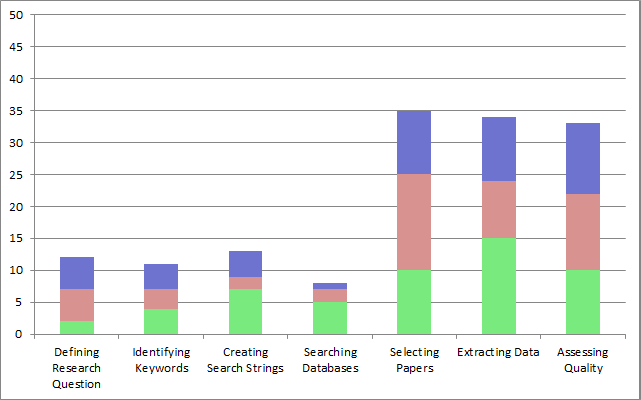
\includegraphics[width=0.48\linewidth]{difficulty.png}
        \label{fig: difficult}
    }
    \subfloat[Most Time Consuming Aspects of SLR Process.]
    {
        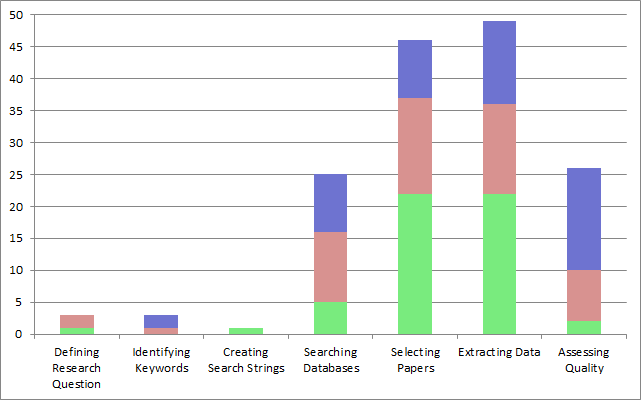
\includegraphics[width=0.48\linewidth]{time.png}
        \label{fig: time}
    }    
    \caption{Data collected from surveys to SLR authors~\cite{carver2013identifying}. {\setlength{\fboxsep}{1pt}\colorbox{green!40}{green}}, {\setlength{\fboxsep}{1pt}\colorbox{red!30}{red}}, and {\setlength{\fboxsep}{1pt}\colorbox{blue!50}{blue}} show the most,   second most, and third most, respectively voted item.}
    \label{fig:barrier}
\end{figure}




\section{Background}
\label{sect: sect2}

% In the modern academic world, before
% attempting new research, it is wise
% to reflect on  what other researchers have done in the same topic area. Finding
% such relevant documents is becoming more difficuly since the number of new publications every year is growing rapidly. For example, on defect prediction, 729 studies were published on IEEE Xplore (http://ieeexplore.ieee.org) during the year of 2005 while 1,564 studies were published during the year of 2015.
% Given this increasingly faster pace of software engineering (SE) research.

Systematic Literature Reviews
(SLRs)  are a well established and widely
applied review method in Software Engineering since Kitchenham, Dyb{\^{a}}, and
J{\o}rgensen first adopted it to support evidence-based software engineering in
2004 and 2005~\cite{kitchenham2004evidence,1377125}. 
Researchers can get a
general idea of current activity in their field of interests by reading the SLR studies. Furthermore, a
deeper understanding of the topic may be gained by conducting an SLR.

An increasing number of SLRs has been conducted since the proposal and revision of the SLR guidelines by Kitchenham in 2007~\cite{keele2007guidelines}. For example, there were 26 SLRs on IEEE Xplore during the year of 2005 and that
number has increased to 137, 199 for the years 2010, 2015 (respectively). Various scholars  suggest that an SLR is required before any research in Software
Engineering is conducted~\cite{keele2007guidelines}.
While this is certainly a good advice,
currently an SLR is
a large, time consuming and complex
task~\cite{hassler2016identification,hassler2014outcomes,carver2013identifying,bowes2012slurp}.

Cost reduction in SLRs is therefore an important topic and will benefit researchers in software engineering community.
Previously we have analyzed the costs of SLRs~\cite{hassler2014outcomes,carver2013identifying}. As shown in Fig.~\ref{fig:barrier}, primary study selection, which is noted as ``selecting papers'' in Fig.~\ref{fig:barrier}, is among the top three most difficult as well as time-consuming aspects in an SLR. Usually, reviewers need to evaluate thousands of studies trying to find dozens of them that are relevant to the
research questions based on their title, abstract, or full text~\cite{bowes2012slurp}. An extreme
example of this is where reviewers sourced over
3,000 studies, and only used 7 of them in their final review~\cite{bezerra2009systematic}.  In terms of actual
cost, Malheiros has documented in~\cite{malheiros2007visual} that it requires 3 hours for one reviewer to review 100 studies.  This implies that it is a month's work for one graduate student to review 3000 studies or three months' work to review 9000 studies. The cost associated with primary study selection has become a serious problem and will continue to grow in the near future as the population of candidates for primary studies increases dramatically. In this paper, we focus on reducing cost in primary study selection only. Our prioritization on the cost reductions of primary study selection is not to discount the effort associated with other parts of the SLR process. There are tools support other components of SLRs and techniques facilitating primary study selection in different approaches. All these techniques (such as Quasi-Gold Standard based search~\cite{zhang2011empirical,zhang2011identifying}, visual text mining~\cite{Felizardo:2014:VAA:2601248.2601252,felizardo2012visual,felizardo2010approach,malheiros2007visual}, and snowballing~\cite{wohlin2014guidelines,jalali2012systematic}) are compatible with works in this paper and a better performance is expected when applied together. This leads to a direction of future work in which the best setting to integrate different techniques will be explored.

There are three main aspects in primary study selection: \textbf{(1)} retrieving initial list of primary studies, \textbf{(2)} excluding irrelevant studies, \textbf{(3)} including missing studies. We focus on excluding irrelevant studies because \textbf{a)} there already exists techniques and tools to facilitate \textbf{(1)} and \textbf{(3)} such as Snowballing~\cite{jalali2012systematic} and StArt~\cite{hernandes2012using}; \textbf{b)} the performance of excluding irrelevant studies can be evaluated using existing SLR publications.































\subsection{Related Work}
\label{sect: Background}




\subsubsection{Software Engineering Tools}

In recent years, various tools have been developed to facilitate SLRs in software engineering community, as summarized in~\cite{marshall2015tools,marshall2014tools,marshall2013tools}. These tools aim at providing support for protocol development~\cite{Molleri:2015:SWA:2745802.2745825,fernandez2010slr,hernandes2012using}, automated search~\cite{Molleri:2015:SWA:2745802.2745825,hernandes2012using}, primary study selection~\cite{Molleri:2015:SWA:2745802.2745825,hernandes2012using,fernandez2010slr,bowes2012slurp}, quality assessment~\cite{fernandez2010slr,bowes2012slurp,Molleri:2015:SWA:2745802.2745825}, data extraction and validation~\cite{Molleri:2015:SWA:2745802.2745825,hernandes2012using,fernandez2010slr,bowes2012slurp}, data synthesis~\cite{Molleri:2015:SWA:2745802.2745825,hernandes2012using,fernandez2010slr,bowes2012slurp},
and report write up~\cite{Molleri:2015:SWA:2745802.2745825,hernandes2012using,fernandez2010slr,bowes2012slurp}. It is extremely helpful to have a tool for managing the whole SLR process. However, the support for primary study selection using these tools is limited (e.g., to tasks such as assigning review jobs to multiple reviewers or to resolving disagreements).
\respto{0e}Hence, we planned to introduce machine learning to assist primary study selection in SE SLRs but before this paper is published, Ros et al.~\cite{ros2017machine} has achieved this in June 2017. While Ros'17~\cite{ros2017machine} provided a wide range of techniques to support both search and selection, it has several limitations such as a) not compared against state-of-the-art techniques form other domain (which are approaches discussed later in Section~\ref{sect: Electronic Discovery} and~\cite{sect: Evidence-based Medicine}); b) not considering any data balancing; c) tested only on one unpublished dataset. 

Visual text mining (VTM) is a technique especially explored in Software Engineering community to support SLR. It is an unsupervised learning method which visualizes the relationship between candidate studies and helps the reviewer to make quick decisions. Malheiros et al.~\cite{malheiros2007visual} first applied VTM to support primary study selection in SLR. In their small-scale experiment (100 candidate studies, 31 of which are ``relevant''), VTM retrieves around 90\% of the ``relevant'' studies by spending about 30\% as much time as manual review. However, VTM requires some prior experience and knowledge of text mining and visualization techniques to use~\cite{bowes2012slurp}, and more case studies with large scale are needed to validate their results. 


Snowballing is another technique attracting much attention in SE SLR research. Given the inherent relevance relationship between a study and its citations, it is of high probability for the citations of (used in backward snowballing) and the studies cite (used in forward snowballing) a known ``relevant'' study to also be ``relevant''~\cite{kitchenham2004evidence}. Jalali and Wohlin~\cite{jalali2012systematic,wohlin2014guidelines} applied backward snowballing to search for primary studies in SE SLRs and found comparably good result as database search. Felizardo et al.~\cite{felizardo2016using} and Wohlin~\cite{wohlin2016second} applied forward snowballing to update SE SLRs and greatly reduced the number studies need to be reviewed comparing to a database search. This paper does not use snowballing since, as mentioned by Wohlin~\cite{wohlin2014guidelines}, snowballing starts with an initial set of relevant papers.
FASTREAD's task is very different: we start with zero relevant papers.



\subsubsection{Legal Electronic Discovery Tools}
\label{sect: Electronic Discovery}

Electronic Discovery (e-discovery) is a part of civil litigation where one party (the producing party), offers up materials which are pertinent to a legal case~\cite{krishna2016bigse}. This involves a review task where the producing party need to retrieve every ``relevant'' document in their possession and turn them over to the requesting party. It is extremely important to reduce the review cost in e-discovery since in a common case, the producing party will need to retrieve thousands of ``relevant'' documents among millions of candidates. Technology-assisted review (TAR) is the technique to facilitate the review process. The objective of TAR is to find as many
of the ``relevant'' documents in a collection as possible, with reasonable cost~\cite{grossman2013}. Various machine learning algorithms have been studied in TAR. So far, in every controlled studies, continuous active learning (Cormack'15) has outperformed others~\cite{cormack2014evaluation,cormack2015autonomy}, which makes it the state-of-the-art method in legal electronic discovery. It has also been selected as a baseline method in the total recall track of TREC 2015~\cite{roegiest2015trec}. Details on continuous active learning will be provided in Section~\ref{sect: Methods}. 

% Interestingly, the relationship between e-discovery and evidence-based medicine have been discussed in~\cite{leasesystematic} but their methods are still diverged. Relying on Grossman and Cormack~\cite{grossman2013} for support, many legal service providers have adopted TAR to facilitate the review process.

% In summary: the state-of-the-art active learning techniques are patient active learning in evidence-based medicine and continuous active learning in e-discovery.

\subsubsection{Evidence-based Medicine Tools}
\label{sect: Evidence-based Medicine}

Systematic literature reviews were first adopted from evidence-based medicine in
2004~\cite{kitchenham2004evidence}. To facilitate citation screening (primary
study selection) in systematic review, many groups of researchers have investigated different types of machine learning algorithms and evaluation mechanisms~\cite{o2015using,paynter2016epc}. 

Cohen et al. first applied text mining techniques to support citation screening and developed several performance metrics (including WSS@95) for assessing the performance of different techniques in 2006~\cite{cohen2006reducing}. While the great contribution of introducing machine learning and text mining into citation screening as well as the proposed performance metrics of Cohen has been widely acknowledged~\cite{o2015using}, most of Cohen's work focused on supervised learning which does not utilize unlabeled data and relies on random sampling to obtain the sufficiently large training set~\cite{cohen2006reducing,cohen2006effective,cohen2010prospective,cohen2011performance}.

Wallace et al. conducted a series of studies
with machine learning techniques, especially active
learning~\cite{wallace2010semi,wallace2010active,wallace2011should,wallace2012deploying,wallace2013active,wallace2013modernizing,nguyen2015combining}. Wallace
first set up a baseline approach called ``patient active learning'' (Wallace'10) for machine learning assisted citation screening~\cite{wallace2010semi}. The performance of patient active learning is good enough (nearly 100\% of the ``relevant''
citations can be retrieved at half of the conventional review cost) to convince
systematic review conductors to adopt machine learning assisted citation
screening. Instead of improving this baseline method, Wallace then focused on other aspects of machine learning assisted citation screening such as introducing external expert knowledge~\cite{wallace2010active}, allocating review tasks to multiple experts~\cite{wallace2011should} or to crowdsourcing workers~\cite{nguyen2015combining}, and building a tool called abstrackr to provide overall support~\cite{wallace2012deploying}. Wallace's work on this topic is of exemplary high-impact and his core algorithm   (on simple expert screening),   is one of the most popular active learning techniques we have found in the evidence-based medical literature. That said, this technique has not been updated since 2010~\cite{wallace2010semi}. In this paper we are focused on the core active learning algorithm for cost minimization. Hence, we do not explore techniques such as Wallace's use of multiple experts (but in future work, we will explore this approach).


More recent work of Miwa et al. explored alternative data balancing and query strategy in 2014~\cite{miwa2014reducing} and proposed a new treatment of Certainty plus Weighting (Miwa'14). Instead of uncertainty sampling in patient active learning (Wallace'10), Miwa found that certainty sampling provides better results in clinical citation screening tasks. Similar conclusion for data balancing method as weighting relevant examples was found to be more effective than aggressive undersampling. Although not stated explicitly, Certainty plus Weighting keeps training until all ``relevant'' studies have been discovered, which differs from the stopping criteria of Wallace'10. Aside from the core algorithm, additional views from latent Dirichlet allocation (LDA) has been found to be potentially useful.


Other work related to machine learning assisted citation screening do not
utilize active learning and active learning. Pure supervised learning requires a sufficiently large training set, which leads to a huge review cost~\cite{cohen2006reducing,adeva2014automatic}. Semi-supervised learning~\cite{liu2016comparative} does not utilize the human reviewers' feedback for updating the model, which leads to a depreciated performance in a long run. As a result, the patient active learning proposed by Wallace et al.~\cite{wallace2010semi} and the Certainty plus Weighting approach by Miwa et al.~\cite{miwa2014reducing} are still considered to be the state-of-the-art method for citation screening in the scenario with no external knowledge and equally expensive reviewers. Details on these two approaches will be provided in Section~\ref{sect: Methods}.


There are also existing tools to support study selection in systematic reviews, e.g. Abstrakr\footnote{http://abstrackr.cebm.brown.edu}~\cite{wallace2012deploying}, EPPI-Reviewer\footnote{http://eppi.ioe.ac.uk/cms/er4/}~\cite{thomas2010eppi}, Rayaan\footnote{http://rayyan.qcri.org/}~\cite{Ouzzani2016}. Useful features can be found in these tools such as a) Rayaan and EPPI-Reviewer: incorporated keyword search in screening; b) Rayaan and EPPI-Reviewer: deduplication; c) Rayaan and EPPI-Reviewer: define inclusion/exclusion criteria by terms; d) Abstrakr: user defined tags; e) all three: assign review tasks to multiple reviewers; f) all three: automatically extract data from PubMed. However, the active learning parts alone in these tools are depreciated. Under the condition that no additional feature (search, tags, define inclusion/exclusion terms) is used, we tried all three tools with one of our dataset-- Hall set (106 relevant in 8911 studies) and after reviewing 1000 studies, only 10 to 15 relevant ones were found, which was very close to a random sampling result without any learning. Since none of these tools are open-source, we cannot tell whether active learning is applied or how/when it is applied in each tool. This motivates us to develop an open source tool which focuses on active learning to support the primary study selection process. Details about our tool will be presented in Section~\ref{sect: tool}.



\section{Technical Details}
\label{sect: Methods}

As mentioned in Section~\ref{sect: Background}, the existing state-of-the-art methods are Wallace'10~\cite{wallace2010semi} (patient active learning), Miwa'14~\cite{miwa2014reducing} (Certainty plus Weighting), and Cormack'15~\cite{cormack2015autonomy} (continuous active learning). All three state-of-the-art methods share the following techniques.

\textbf{Support vector machines (SVM)} are a well-known and widely used classification technique. The idea behind is to map input data to a high-dimension feature space and then construct a linear decision plane in that feature space~\cite{cortes1995support}. Linear SVM~\cite{joachims2006training} has been proved to be a useful model in SE text mining~\cite{krishna2016bigse} and is applied in the state-of-the-art active learning methods of both evidence-based medicine and electronic discovery~\cite{miwa2014reducing,wallace2010semi,cormack2014evaluation}. \respto{1h}One drawback of SVM is its poor interpretability as compared to classifiers like decision trees. However, SVM is still a perfect fit here since the model itself is not important as long as it could provide a relative ranking of literature.

\textbf{Active learning} is a cost-aware machine learning algorithm where labels of training data can be acquired with certain costs. The key idea behind active learning is that a machine learning algorithm can perform better with less
training if it is allowed to choose the data from which it learns~\cite{settles2012active}. There are several scenarios active learning is applied to, such as membership query synthesis, stream-based selective sampling, and pool-based sampling~\cite{settles2010active}. There are also different query strategies of active learning, such as uncertainty sampling, query-by-committee, expected model change, expected error reduction, variance reduction, and density-weighted methods~\cite{settles2010active}. Here, we will briefly introduce one scenario and two query strategies, which will be used in our later experiments and discussions.
 

\respto{1g}Figure~\ref{fig:SVM} shows a simple demonstration of an SVM active-learner.
For simplificty sake, this demonstration assumes that the data has    two features (shown in that figure as the horizontal and vertical axis). 
 In that figure, ``$O$'' is the minority class, ``relevant'' studies in SLR. ``$O$''s in blue are studies already identified as ``relevant'' (included) by human reviewers. ``$X$'' is the majority class, ``irrelevant'' studies in SLR. ``$X$''s in red are studies already identified as ``irrelevant'' (excluded) by human reviewers (note that in (c), some red ``$X$''s are removed from the training set by aggressive undersampling). Markers in gray are the unlabeled studies (studies have not been reviewed yet), and black line is SVM decision plane. In (b) Weighting balances the training data by putting more weight on the minority class examples. In (c), aggressive undersampling balances the training data by throwing away majority class examples closest to the old decision plane in (a). When deciding which studies to be reviewed next, uncertainty sampling returns the unlabeled examples closest to the decision plane (U) while certainty sampling returns the unlabeled examples furthest to the decision plane from the bottom-left side (C).


\begin{figure}[!t]
    \centering
    \subfloat[No data balancing]
    {
        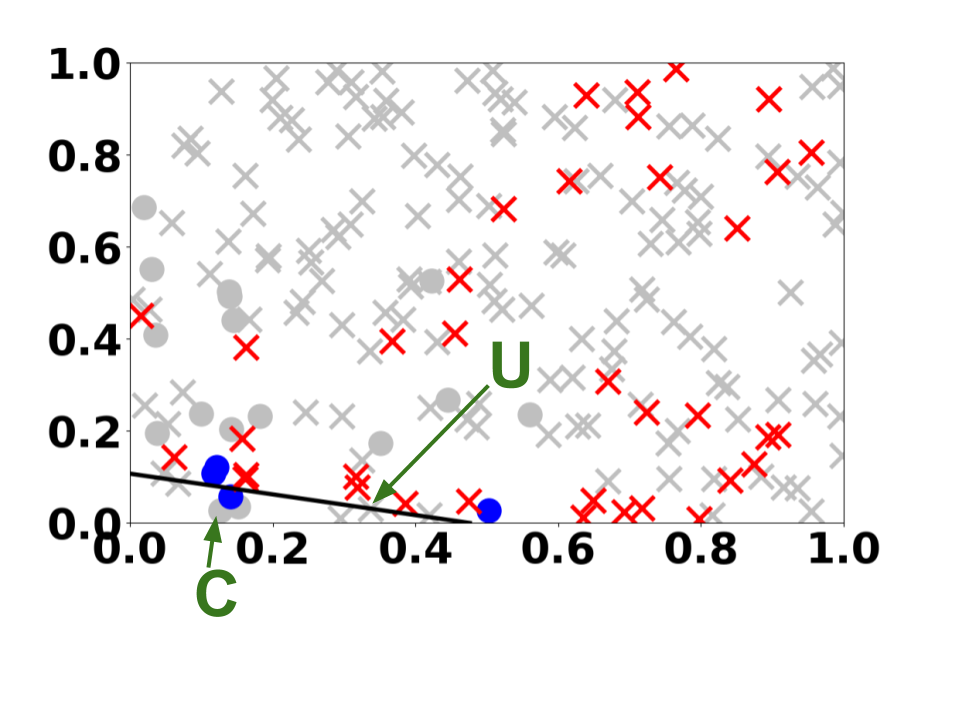
\includegraphics[width=0.33\linewidth]{simu22.png}
        \label{fig:nobal}
    }
    \subfloat[With weighting]
    {
        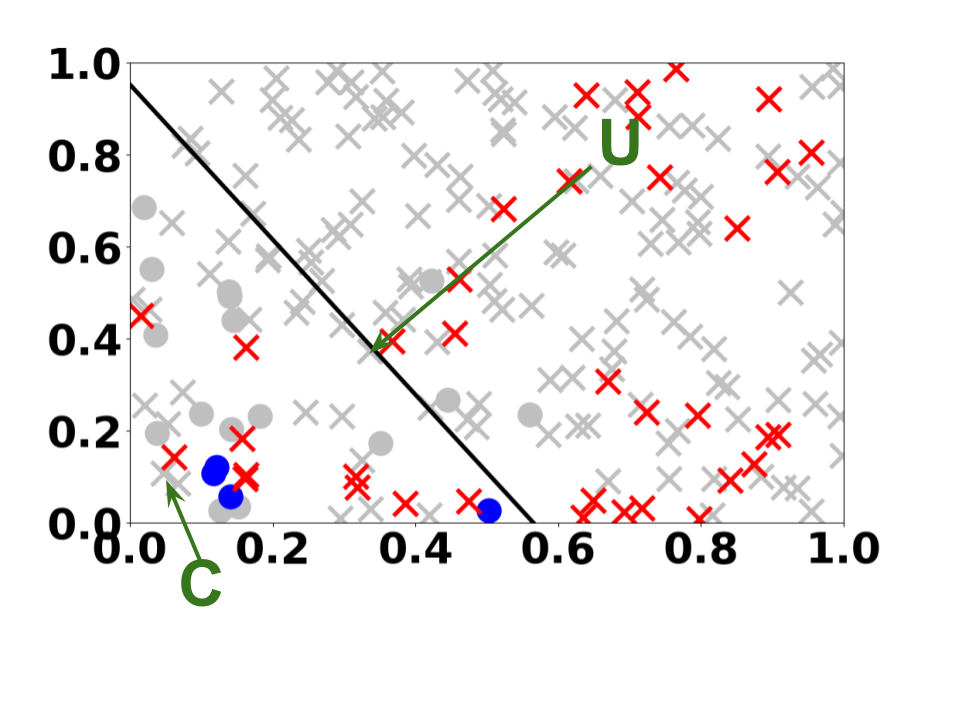
\includegraphics[width=0.33\linewidth]{simu24.png}
        \label{fig:weighting}
    }
    \subfloat[With aggressive undersampling. ]
    {
        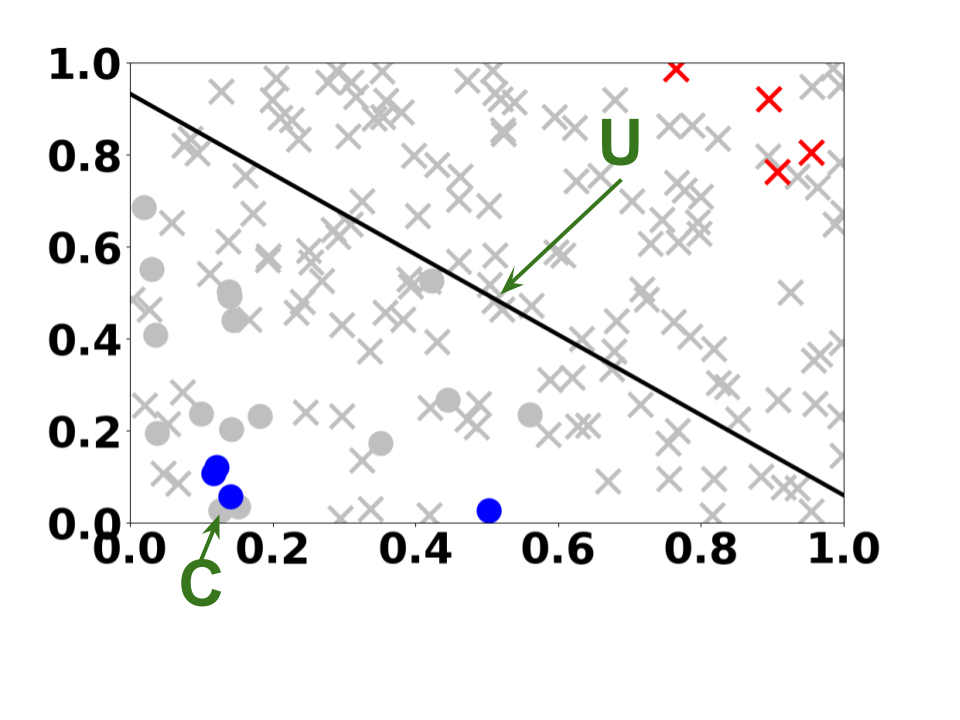
\includegraphics[width=0.33\linewidth]{simu23.png}
        \label{fig:aggress}
    }
    \caption{Active learning with SVM and different data balancing techniques.}
    \label{fig:SVM}
\end{figure}

By analyzing the differences between the state-of-the-art methods, we identified the following key components in solving the problem with active learning and linear SVM

\vspace{3mm}
\noindent
{\em When to start training}: 
\begin{itemize}
\item \textbf{P} stands for ``patient''. As suggested by Wallace et al.~\cite{wallace2010semi}, ``hasty generation'', which means start training with too few relevant examples, may leads to deteriorate performance. The algorithm keeps random sampling until a sufficient number of ``relevant'' studies retrieved. In our experiments, the sufficient number of ``relevant'' studies retrieved is set to $5$, which means when at least $5$ ``relevant'' studies have been retrieved by random sampling, the algorithm goes into next stage. Wallace'10~\cite{wallace2010semi} and Miwa'14~\cite{miwa2014reducing} use \textbf{P} for when to start training.
\item
\textbf{H} is the opposite. The algorithm stops random sampling as long as {\em ONE} ``relevant'' studies are retrieved, as suggested in Cormack'15~\cite{cormack2014evaluation,cormack2015autonomy}.
\end{itemize}
{\em Which document to query next}: 
\begin{itemize}
\item
\textbf{U} stands for ``uncertainty sampling''. The algorithm utilizes uncertainty sampling to build the classifier, where unlabeled examples closest to the SVM decision plane are sampled for query (U in Figure~\ref{fig:SVM}). Wallace'10~\cite{wallace2010semi} uses \textbf{U} for Query strategy.
\item
\textbf{C} stands for ``certainty sampling''. The algorithm utilizes certainty sampling to build the classifier, where unlabeled examples furthest to the SVM decision plane and lie in the ``relevant'' side are sampled for query (C in Figure~\ref{fig:SVM}). Miwa'14~\cite{miwa2014reducing} and Cormack'15~\cite{cormack2014evaluation,cormack2015autonomy} use \textbf{C} for query strategy.
\end{itemize}
\newpage {\em Whether to stop training (or not)}: 
\begin{itemize}
\item
\textbf{S} stands for ``stop training''. The algorithm stops training
once the classifier is stable. In our experiments, the classifier is treated as stable once more than $30$ ``relevant'' studies have been retrieved as training examples. Wallace'10~\cite{wallace2010semi} uses \textbf{S} for whether to stop training.
\item
\textbf{T} stands for ``continue training''. The algorithm never stops
training as suggested in Cormack'15~\cite{cormack2015autonomy} and Miwa'14~\cite{miwa2014reducing}. If query strategy is \textbf{U}, algorithm switches to certainty sampling after classifier is stable but training never stops.
\end{itemize}
{\em How to balance the training data}: 
\begin{itemize}
\item
\textbf{N} stands for ``no data balancing''. The algorithm does not balance the training data (demonstrated in Figure~\ref{fig:nobal}) as suggested by Cormack'15~\cite{cormack2015autonomy}.
\item
\textbf{A} stands for ``aggressive undersampling''. The algorithm utilizes aggressive undersampling\footnote{Aggressive undersampling throws away majority (irrelevant) training examples closest to SVM decision plane until reaching the same number of minority (relevant) training examples. A demonstration is shown in Figure~\ref{fig:aggress}.} after classifier is stable, as suggested by Wallace'10~\cite{wallace2010semi}.
\item
\textbf{W} stands for ``Weighting''. The algorithm utilizes Weighting\footnote{Weighting assigns different weight to each class, $W_R = 1/|L_R|,\,W_I = 1/|L_I|$, when training SVM. A demonstration is shown in Figure~\ref{fig:weighting}. $L_R$ is defined in Figure~\ref{fig:Problem Statement}.} for data balancing (before and after the classifier is stable), as suggested by Miwa'14~\cite{miwa2014reducing}.
\item
\textbf{M} stands for ``mixing of Weighting and aggressive undersampling''. Weighting is applied before the classifier is stable while aggressive undersampling is applied after the classifier is stable. This treatment comes from the observation that ``Weighting'' performs good in early stages while ``aggressive undersampling'' performs good in late stages.
\end{itemize}
By combining different approaches, we ended up with 32 possible treatments including the state-of-the-art methods including:
\begin{itemize}
\item
The \textbf{PUSA} approach advocated by Wallace'10~\cite{wallace2010semi};
\item
The \textbf{PCTW} approach advocated by Miwa'14~\cite{miwa2014reducing};
\item
The \textbf{HCTN} approach advocated by Cormack'15~\cite{cormack2015autonomy}.
\end{itemize}
Pseudo code for the 32 machine learning treatments are shown in Algorithm~\ref{alg:alg1}. Along with the current standard procedure as a baseline approach:
\begin{itemize}
\item
\textbf{Linear Review}: no machine learning, query studies in a random order,
\end{itemize}
all the 32 machine learning treatments are tested and compared in Section~\ref{sect: Experiments}.


\section{Experiments}
\label{sect: Experiments}

This section describes the experimental procedures that we used to evaluate the treatments described in Section~\ref{sect: Methods}. 

\subsection{Performance Metrics}
\label{sect: Performance Metrics}

As shown in Figure~\ref{fig:Problem Statement}, the problem to be solved is multi-objective. The performance of each algorithm is thus evaluated by its \textbf{recall ($|L_R|/|R|$)} vs. \textbf{studies reviewed ($|L|$)} curve. This performance metrics is suggested by~\cite{cormack2015autonomy,cormack2014evaluation,tredennick2015} and best fits the objectives of excluding 

\noindent
\begin{minipage}[t]{.54\textwidth}
\vspace{0pt}
\centering
\begin{algorithm}[H]
\footnotesize
\SetKwInOut{Input}{Input}
\SetKwInOut{Output}{Output}
\SetKwInOut{Parameter}{Parameter}
\SetKwRepeat{Do}{do}{while}
\Input{$E$, set of all candidate studies\\$R$, set of ground truth relevant studies\\$AL$, algorithm code, e.g. \textbf{PUSA} for \\Wallace'10 treatment}
\Output{$L_R$, set of included studies}
\BlankLine

$L\leftarrow 0$\; $L_R\leftarrow 0$\; $\neg L\leftarrow E$\; 

\BlankLine
\tcp{Keep reviewing until stopping rule satisfied}
\While{$|L_R| < 0.95|R|$}{
    \tcp{Start training or not}
    \eIf{$|L_R| \geq Enough(AL)$}{
        \If{\textbf{T} $\in AL$ {\bf or} $NotStable(L_R)$}{
            $CL\leftarrow Train(AL,L)$\;
        }
        \tcp{Query next}
        $x\leftarrow Query(AL,CL,\neg L,LR)$\;
    }{
        \tcp{Random Sampling}
        $x\leftarrow Random(\neg L)$\;
    }
    \tcp{Simulate review}
    $L\leftarrow L \cup x$\;
    $\neg L\leftarrow \neg L \setminus x$\;
    \If{$x\in R$}{
        $L_R\leftarrow L_R \cup x$\;
    }
}
\Return{$L_R$}\;
\caption{Psuedo Code}\label{alg:alg1}
\end{algorithm}
\end{minipage}\hfill
\begin{minipage}[t]{.46\textwidth}
\vspace{0pt}
\centering \small
~~~~~~~~\begin{tabular}{p{1.8in}}\hline
\rowcolor{gray!10}
The algorithm on this page use
the following notation. 
\begin{itemize}
\item
$E$: the set of all candidate studies (returned from search);
\item
$R\subset E$: the set of ground truth relevant studies;
\item
$I=E\setminus R$: the set of ground truth irrelevant studies;
\item
$L\subset E$: the set of labeled/reviewed studies, each review reveals whether a study $x\in R$, but incurs a cost;
\item
$\neg L=E\setminus L$: the set of unlabeled/unreviewed studies;
\item
$L_R=L\cap R$: the identified relevant (included) studies;
\item
$L_I=L\cap I$: the identified irrelevant (excluded) studies.
\end{itemize}
The general form of the excluding irrelevant studies problem can be described as following: start with $L=\emptyset$, prioritize which studies to be reviewed so as to maximize $|L_R|$ while minimizing $|L|$ (identify more relevant studies with less cost). \hline
  \end{tabular}
  \captionof{figure}{Notations and Problem Description}
  \label{fig:Problem Statement}
\end{minipage}
\SetAlgoFuncName{Support functions for Algorithm~\ref{alg:alg1}}{Function}
\begin{function}[H]
% \setcounter{AlgoLine}{15}
\footnotesize
$t1\leftarrow 5$\; $t2\leftarrow 30$\;
\BlankLine
% \tcp{When to start training}
\Fn{Enough(AL)}{
    \uIf{\textbf{P} $\in AL$}{
        \Return{$t1$}\;
    }
    \uElseIf{\textbf{H} $\in AL$}{
        \Return{$1$}\;
    }
    \Else{
        \Return{$\infty$}\;
    }
}
\BlankLine
% \tcp{Model is stable or not}
\Fn{NotStable($L_R$)}{
    \lIf{$|L_R|\geq t2$}{
        \Return{False}
    }
    \lElse{
        \Return{True}
    }
}
\BlankLine
\Fn{Train(AL,L)}{
    \If{\textbf{W} $\in AL$ \textbf{or} \textbf{M} $\in AL$}{
        \tcp{Train linear SVM with Weighting}
        $CL\leftarrow SVM(L,kernel=linear,class\_weight=balanced)$\;
    }
    \Else{
        \tcp{Train linear SVM}
        $CL\leftarrow SVM(L,kernel=linear)$\;
    }
    \If{\textbf{A} $\in AL$ \textbf{or} \textbf{M} $\in AL$}{
        \tcp{Aggressive undersampling}
        $L_I\leftarrow L\setminus L_R$\;
        $tmp\leftarrow L_I[argsort(CL.decision\_function(L_I))[:|L_R|]]$\;
        $CL\leftarrow SVM(L_R \cup tmp,kernel=linear)$\;
    }
    \Return{$CL$}\;
}
\BlankLine
\Fn{Query(AL,CL,\neg L,$L_R$)}{
    \eIf{\textbf{U} $\in AL$ \textbf{and} $NotStable(L_R)$}{
        \tcp{Uncertainty Sampling}
        $x\leftarrow \neg L[argsort(abs(CL.decision\_function(\neg L)))[0]]$\;
    }{
        \tcp{Certainty Sampling}
        $x\leftarrow \neg L[argsort(CL.decision\_function(\neg L))[-1]]$\;
    }
    \Return{$x$}\;
}
% \NoCaptionOfAlgo
\caption{()}
\end{function}






% \begin{algorithm}[!htbp]
% \footnotesize
% \SetKwInOut{Input}{Input}
% \SetKwInOut{Output}{Output}
% \SetKwInOut{Parameter}{Parameter}
% \SetKwRepeat{Do}{do}{while}
% \Input{$P$, set of all candidate studies\\$R$, set of ground truth relevant studies\\$AL$, algorithm code, e.g. \textbf{PUSA} for Wallace'10}
% \Output{$L_R$, set of included studies}
% \BlankLine

% $L\leftarrow 0$\; $L_R\leftarrow 0$\; $U\leftarrow P$\; $t1\leftarrow 5$\; $t2\leftarrow 30$\;

% \BlankLine
% \tcp{Keep reviewing until stopping rule satisfied}
% \While{$|L_R| < 0.95|R|$}{
%     \tcp{Start training or not}
%     \eIf{$|L_R| \geq Enough(AL)$}{
%         \If{\textbf{T} $\in AL$ {\bf or} $NotStable(L_R)$}{
%             $CL\leftarrow Train(AL,L)$\;
%         }
%         \tcp{Query next}
%         $x\leftarrow Query(AL,CL,U,LR)$\;
%     }{
%         \tcp{Random Sampling}
%         $x\leftarrow Random(U)$\;
%     }
%     \tcp{Simulate review}
%     $L\leftarrow L \cup x$\;
%     $U\leftarrow U \setminus x$\;
%     \If{$x\in R$}{
%         $L_R\leftarrow L_R \cup x$\;
%     }
% }
% \Return{$L_R$}\;
% \BlankLine
% \tcp{When to start training}
% \Fn{Enough(AL)}{
%     \uIf{\textbf{P} $\in AL$}{
%         \Return{$t1$}\;
%     }
%     \uElseIf{\textbf{H} $\in AL$}{
%         \Return{$1$}\;
%     }
%     \Else{
%         \Return{$\infty$}\;
%     }
% }
% \BlankLine
% \tcp{Model is stable or not}
% \Fn{NotStable($L_R$)}{
%     \lIf{$|L_R|\geq t2$}{
%         \Return{False}
%     }
%     \lElse{
%         \Return{True}
%     }
% }
% \BlankLine
% \Fn{Train(AL,L)}{
%     \If{\textbf{W} $\in AL$ \textbf{or} \textbf{M} $\in AL$}{
%         \tcp{Train linear SVM with Weighting}
%         $CL\leftarrow SVM(L,kernel=linear,class\_weight=balanced)$\;
%     }
%     \Else{
%         \tcp{Train linear SVM}
%         $CL\leftarrow SVM(L,kernel=linear)$\;
%     }
%     \If{\textbf{A} $\in AL$ \textbf{or} \textbf{M} $\in AL$}{
%         \tcp{Aggressive undersampling}
%         $L_U\leftarrow L\setminus L_R$\;
%         $tmp\leftarrow L_U[argsort(CL.decision\_function(L_U))[:|L_R|]]$\;
%         $CL\leftarrow SVM(L_R \cup tmp,kernel=linear)$\;
%     }
%     \Return{$CL$}\;
% }
% \BlankLine
% \Fn{Query(AL,CL,U,$L_R$)}{
%     \eIf{\textbf{U} $\in AL$ \textbf{and} $NotStable(L_R)$}{
%         \tcp{Uncertainty Sampling}
%         $x\leftarrow U[argsort(abs(CL.decision\_function(U)))[0]]$\;
%     }{
%         \tcp{Certainty Sampling}
%         $x\leftarrow U[argsort(CL.decision\_function(U))[-1]]$\;
%     }
%     \Return{$x$}\;
% }
% \caption{Psuedo Code}\label{alg:alg}
% \end{algorithm}



% \subsection{Problem}
% \label{sect: problem}

% The general form of the excluding irrelevant studies problem can be considered as a needle in a haystack problem with:
% \begin{itemize}
% \item
% $P$: the set of all candidate studies (returned from search);
% \item
% $R\subset P$: the set of ground truth relevant studies;
% \item
% $I=P\setminus R$: the set of ground truth irrelevant studies;
% \item
% $L\subset P$: the set of labeled/reviewed studies, each review reveals whether a study $x\in R$, but incurs a cost;
% \item
% $U=P\setminus L$: the set of unlabeled/unreviewed studies;
% \item
% $L_R=L\cap R$: the identified relevant (included) studies;
% \item
% $L_I=L\cap I$: the identified irrelevant (excluded) studies.
% \end{itemize}
% Start with $L=\o$, prioritize which studies to be reviewed so as to maximize $|L_R|$ while minimizing $|L|$ (identify more relevant studies with less cost). 



\noindent
irrelevant studies problem. To enable a statistical analysis of the performances, the \textbf{recall} vs. \textbf{studies reviewed} curve is cut by a $0.95$ \textbf{recall} line where \textbf{studies reviewed} ($|L|$) when reaching $0.95$ \textbf{recall} ($|L_R|\geq 0.95|R|$) is used to assess performances. The reason behind 
$0.95$ \textbf{recall} is that a) $1.00$ \textbf{recall} can never be guaranteed by any text mining method unless all the candidate studies are reviewed; b) $0.95$ \textbf{recall} is usually considered acceptable in evidence-based medicine~\cite{cohen2011performance,cohen2006reducing,o2015using} despite the fact that there might still be ``relevant'' studies missing~\cite{shemilt2016use}. As a result, two metrics are used for evaluation:
\begin{itemize}
\item
X95 = $\min \{|L| \mid |L_R|\geq0.95 |R|\}$
\item
WSS@95 = $0.95-\text{X95}/|P|$.
\end{itemize}
Note that one algorithm is better than the other if its X95 is smaller or WSS@95~\cite{cohen2011performance} is larger.


\subsection{Datasets}
\label{sect: datasets}


Although a large number of SLRs are published every year, there is no dataset clearly documenting the details in primary study selection. As a result, three datasets are created reverse-engineering existing SLRs and being used in this study to simulate the process of excluding irrelevant studies. The three datasets are named after the authors of their original publication source-- Wahono dataset from Wahono et al. 2015~\cite{wahono2015systematic}, Hall dataset from Hall et al. 2012~\cite{hall2012systematic}, and Radjenovi{\'c} dataset from Radjenovi{\'c} et al. 2013~\cite{radjenovic2013software}. 

For each of the datasets, the search string \textbf{S} and the final inclusion list \textbf{F} from the original publication are used for the data collection. We retrieve the initial candidate collection \textbf{E} from IEEE Xplore with the search string (slightly modified to meet the requirement of IEEE Xplore). Then make a final list of inclusion \textbf{R} as \textbf{R} = \textbf{F} $\cap$ \textbf{E}. Here, for simplicity reason we only extract candidate studies from IEEE Xplore. We will explore possibilities for efficiently utilizing multiple data sources in the future work but in this paper, without loss of generality, we only extract initial candidate list from single data source. In this way, we created three datasets that reasonably resemble real SLR selection results assuming that any study outside the final inclusion list \textbf{F} is irrelevant to the original SLRs. A summary of the created datasets is presented in Table~\ref{tab: number}.

Apart from the three created datasets, one dataset (Kitchenham) is provided directly by the author of Kitchenham et al. 2010~\cite{kitchenham2010systematic} and includes two levels of relevance information. In general, only the ``content relevant'' labels are used in experiments for a fair comparison with other datasets. Additionally, the ``abstract relevant'' labels are used for detailed review cost analysis in RQ3. Summary of Kitchenham dataset is also presented in Table~\ref{tab: number}.

All the above datasets are available on-line at Seacraft, Zenodo\footnote{\em https://doi.org/10.5281/zenodo.837298}.

\begin{table}
\caption{Descriptive statistics for experimental datasets}
\label{tab: number}
\begin{center}
\begin{tabular}{ |l|c|c|c|c| }
  \hline
   Datasets & \multicolumn{2}{|c|}{Generated} & \multicolumn{2}{|c|}{Original} \\
  \cline{2-5}
  & \#Candidate $|$\textbf{E}$|$ & \#Relevant $|$\textbf{R}$|$& \#Candidate & \#Relevant $|$\textbf{F}$|$\\
  \hline
  Wahono & 7002 & 62 & 2117 & 72\\
  \hline
  Hall & 8911 & 106 & 2073 & 136 \\
  \hline
  Radjenovi{\'c} & 6000 & 48 & 13126 & 106\\
  \hline
  Kitchenham & 1704 & 44 (132) & 1704 & 44 (132) \\
  \hline
\end{tabular}
\end{center}
{\footnotesize Our datasets are generated using information in the original SLR literature. Our candidate studies are retrieved by applying similar if not the same the search string from original SLR literature and search in IEEE Xplore. The set of our relevant studies is the intersection of the set of our candidate studies and the set of final included studies in the original SLR literature. Kitchenham dataset is different as it is provided directly by Kitchenham and it has two level of relevance labels-- 132 relevant studies by title and abstract review and within which, 44 relevant studies by content review.}
\end{table}

There is no human activity involved in these experiments, when asked for a label, the true label in the dataset is queried instead of a human reviewer. As a result, each experiment can be repeated with different random seed to capture variances and also makes reproducing the experiments possible. Each experiment is a simulation of one specific treatment on one dataset.

\subsection{Controlled Variables}
\label{sect: Controlled Variables}

For the sake of a fair comparison, different treatments in Section~\ref{sect: Methods} share an identical set of controlled variables including preprocessing, featurization and classifier. 

Each candidate study in the initial list is first tokenized by stop words removal after concatenating its title and abstract. After tokenization, the bag of words are featurized into a term frequency vector. Then, reduce the dimensionality of the term frequency vector with to keep only $M=4000$ of the terms with highest tf-idf\footnote{For term $t$ in document $d$, $Tfidf(t, d)=w^t_d\times (\log \frac{|D|}{\sum_{d\in D} sgn(w^t_d)}+1)$ where $w^t_i$ is the term frequency of term $t$ in document $d$. For term $t$, $Tfidf(t) = \sum_{d\in D} Tfidf(t,d) = \sum_{d\in D} w^t_d \times (\log \frac{|D|}{\sum_{d\in D} sgn(w^t_d)}+1)$ and is used for feature selection.} score and normalize the hashed matrix by its L2 norm each row at last. TfidfVectorizer in scikit-learn is utilized for the above preprocessing and featurization steps. Alternatives such as stemming, LDA~\cite{blei2003latent}, paragraph vectors~\cite{le2014distributed} require further exploration and are scheduled in our future works. All 32 treatments use the same classifier-- linear SVM from scikit-learn.



\section{Results}
\label{subsect: Results}


All the following results were generated from 30 repeats
simulations, using different random number seeds from each simulation.
As shown below, all our results
are reported in terms of medians (50th percentile) and iqrs ((75-25)th percentile).

\begin{table*}
\caption{Scott-Knott analysis for number of studies reviewed/ work saved over sampling to reach $95\%$ recall}
\label{tab: scottknott}


\begin{center}
\parbox{.49\linewidth}{
\centering
{\scriptsize \begin{tabular}{l@{~~~}l@{~~~}r@{~~~}r@{~~~}r@{~~~}r}
\arrayrulecolor{lightgray}
\multicolumn{2}{l}{\textbf{Wahono}}  & \multicolumn{2}{c}{\textbf{X95}} & \multicolumn{2}{c}{\textbf{WSS@95}}\\\hline
\textbf{Rank} & \textbf{Treatment} & \textbf{Median} & \textbf{IQR} & \textbf{Median} & \textbf{IQR} \\\hline
\rowcolor{green!40}
  1 &         HUTM &    670  &  230 & 0.85 & 0.04 \\
  1 &         HCTM &    740  &  220 & 0.84 & 0.03 \\
\hline  2 &         HUTA &    780  &  140 & 0.84 & 0.02 \\
  2 &         HCTW &    790  &  90 & 0.84 & 0.02 \\
  2 &         HUTW &    800  &  110 & 0.84 & 0.02 \\
  2 &         HCTA &    800  &  140 & 0.83 & 0.02 \\
\hline  3 &         PCTM &    1150  &  450 & 0.78 & 0.07  \\
  3 &         PUTM &    1180  &  420 & 0.78 & 0.07 \\
  3 &         PCTA &    1190  &  340 & 0.78 & 0.05 \\
  3 &         PUTA &    1190  &  340 & 0.78 & 0.05 \\
\rowcolor{red!30}
  3 &         PCTW &    1210  &  350 &  0.78 & 0.06 \\
  3 &         PUTW &    1220  &  370 &  0.77 & 0.06 \\
\hline  4 &         HUSM &    1410  &  400 & 0.75 & 0.06 \\
\hline  5 &         HUSA &    1610  &  370 & 0.72 & 0.07 \\
\hline  6 &         PUSM &    1810  &  370 & 0.69 & 0.06 \\
\rowcolor{red!30}
  6 &         PUSA &    1910  &  700 & 0.67 & 0.10 \\
\hline  7 &         HUSW &    2220  &  400 & 0.63 & 0.06 \\
  7 &         PUSW &    2240  &  360 & 0.63 & 0.06 \\
\hline  8 &         HUTN &    2700  &  40 & 0.56 & 0.01 \\
\rowcolor{red!30}
  8 &         HCTN &    2720  &  40 & 0.56 & 0.01 \\
  8 &         PCSW &    2860  &  1320 & 0.54 & 0.20 \\
  8 &         PCSM &    2860  &  1320 & 0.54 & 0.20 \\
  8 &         PCTN &    2850  &  1130 & 0.54 & 0.17 \\
  8 &         PUTN &    2850  &  1130 & 0.54 & 0.17 \\
\hline  9 &         PCSN &    3020  &  1810 & 0.51 & 0.26 \\
  9 &         PCSA &    3020  &  1810 & 0.51 & 0.26 \\
\hline 10 &         HUSN &    4320  &  110 &  0.33 & 0.03 \\
 10 &         PUSN &    4370  &  1290 & 0.32 & 0.19 \\
 \rowcolor{blue!50}
\hline 11 &       linear &    6650  &  0 & 0 & 0 \\
 11 &         HCSA &    6490  &  2760 & -0.01 & 0.39 \\
 11 &         HCSN &    6490  &  2760 & -0.01 & 0.39 \\
 11 &         HCSM &    6490  &  3110 & -0.01 & 0.44 \\
 11 &         HCSW &    6490  &  3110 & -0.01 & 0.44 \\
\hline \end{tabular}}
}
\parbox{.49\linewidth}{
\centering
{\scriptsize \begin{tabular}{l@{~~~}l@{~~~}r@{~~~}r@{~~~}r@{~~~}r}
\arrayrulecolor{lightgray}
\multicolumn{2}{l}{\textbf{Hall}}  & \multicolumn{2}{c}{\textbf{X95}} & \multicolumn{2}{c}{\textbf{WSS@95}}\\\hline
\textbf{Rank} & \textbf{Treatment} & \textbf{Median} & \textbf{IQR} & \textbf{Median} & \textbf{IQR} \\\hline
  1 &         HUTW &    350  &  80 & 0.91 & 0.01 \\
  1 &         HUTA &    360  &  140 & 0.91 & 0.02 \\
  \rowcolor{green!40}
  1 &         HUTM &    360  &  140 & 0.91 & 0.02 \\
  1 &         HCTW &    370  &  50 & 0.91 & 0.01 \\
\hline  2 &         HCTM &    400  &  90 & 0.90 & 0.01 \\
  2 &         HCTA &    410  &  140 & 0.90 & 0.02 \\
  2 &         HUTN &    430  &  100 & 0.90 & 0.01 \\
  \rowcolor{red!30}
  2 &         HCTN &    460  &  70 & 0.90 & 0.01 \\
\hline  3 &         HUSM &    630  &  160 & 0.88 & 0.03 \\
\rowcolor{red!30}
  3 &         PCTW &    640  &  190 & 0.88 & 0.02 \\
  3 &         PUTW &    640  &  220 & 0.88 & 0.03 \\
\hline  4 &         PCTN &    680  &  210 & 0.87 & 0.03 \\
  4 &         PUTN &    680  &  200 & 0.87 & 0.03 \\
  4 &         PUTM &    690  &  230 & 0.87 & 0.03 \\
  4 &         PCTA &    730  &  260 & 0.87 & 0.03 \\
  4 &         PCTM &    720  &  230 & 0.87 & 0.03 \\
  4 &         PUTA &    730  &  230 & 0.87 & 0.03 \\
\hline  5 &         HUSW &    790  &  320 & 0.86 & 0.04 \\
  5 &         HUSA &    790  &  200 & 0.86 & 0.03 \\
  5 &         PUSW &    840  &  280 & 0.86 & 0.03 \\
  5 &         PUSM &    860  &  320 & 0.85 & 0.04 \\
  \rowcolor{red!30}
  5 &         PUSA &    970  &  310 & 0.84 & 0.04 \\
\hline  6 &         PCSW &    1560  &  580 & 0.77 & 0.07 \\
  6 &         PCSM &    1560  &  580 & 0.77 & 0.07 \\
\hline  7 &         PUSN &    1680  &  1390 & 0.76 & 0.18 \\
  7 &         PCSN &    1990  &  690 & 0.72 & 0.09 \\
  7 &         PCSA &    1990  &  690 & 0.72 & 0.09 \\
\hline  8 &         HUSN &    2270  &  1230 & 0.69 & 0.16 \\
\hline  9 &         HCSA &    7500  &  5170 & 0.03 & 0.58 \\
  9 &         HCSN &    7500  &  5170 & 0.03 & 0.58 \\
   \rowcolor{blue!50}
  9 &       linear &    8464  &  0 & 0 & 0 \\
  9 &         HCSM &    8840  &  5340 & -0.04 & 0.60 \\
  9 &         HCSW &    8840  &  5340 & -0.04 & 0.60 \\
\hline \end{tabular}}
}


\parbox{.49\linewidth}{
\centering
{\scriptsize \begin{tabular}{l@{~~~}l@{~~~}r@{~~~}r@{~~~}r@{~~~}r}
\arrayrulecolor{lightgray}
\multicolumn{2}{l}{\textbf{Radjenovi{\'c}}}  & \multicolumn{2}{c}{\textbf{X95}} & \multicolumn{2}{c}{\textbf{WSS@95}}\\\hline
\textbf{Rank} & \textbf{Treatment} & \textbf{Median} & \textbf{IQR} & \textbf{Median} & \textbf{IQR} \\\hline
\rowcolor{green!40}
  1 &         HUTM &    680   &  180  & 0.83 & 0.03 \\
  1 &         HCTM &    780   &  130  & 0.82 & 0.02 \\
  1 &         HCTA &    790   &  180  & 0.82 & 0.03 \\
  1 &         HUTA &    800   &  180  & 0.82 & 0.03 \\
\hline  2 &         HUSA &    890   &  310  & 0.80 & 0.06 \\
  2 &         HUSM &    890   &  270  & 0.80 & 0.05 \\
\hline  3 &         HUTW &    960   &  80  & 0.79 & 0.02 \\
  3 &         HCTW &    980   &  60  & 0.79 & 0.01 \\
  3 &         HUSW &    1080   &  410  & 0.77 & 0.07 \\
\hline  4 &         PCTM &    1150   &  270  & 0.76 & 0.05 \\
  4 &         PUTM &    1150   &  270  & 0.76 & 0.05 \\
\hline  5 &         HUTN &    1250   &  100  &  0.74 & 0.02 \\
  5 &         PCTA &    1260   &  210  & 0.74 & 0.05 \\
  5 &         PUTA &    1260   &  210  & 0.74 & 0.05 \\
  \rowcolor{red!30}
  5 &         HCTN &    1270   &  70  & 0.74 & 0.02 \\
  5 &         PUSM &    1250   &  400  & 0.74 & 0.07 \\
  5 &         PUSW &    1250   &  450  & 0.73 & 0.08 \\
  5 &         PUTW &    1350   &  310  & 0.72 & 0.06 \\
\rowcolor{red!30}
  5 &         PCTW &    1370   &  310  & 0.72 & 0.06 \\
  \rowcolor{red!30}
  5 &         PUSA &    1400   &  490  & 0.71 & 0.09 \\
\hline  6 &         HUSN &    1570   &  300  & 0.69 & 0.05 \\
  6 &         PCTN &    1600   &  360  & 0.68 & 0.06 \\
  6 &         PUTN &    1600   &  360  & 0.68 & 0.06 \\
\hline  7 &         PUSN &    1890   &  320  &  0.64 & 0.06 \\
\hline
  8 &         PCSW &    2250   &  940  & 0.57 & 0.20 \\
  8 &         PCSM &    2250   &  940  & 0.57 & 0.20 \\
\hline  9 &         PCSN &    2840   &  1680  & 0.47 & 0.31 \\
  9 &         PCSA &    2840   &  1680  & 0.47 & 0.31 \\
\hline 10 &         HCSA &    5310   &  2140  & 0.07 & 0.36 \\
 10 &         HCSN &    5310   &  2140  & 0.07 & 0.36  \\
 10 &         HCSM &    5320   &  2200  &  0.02 & 0.37  \\
 10 &         HCSW &    5320   &  2200  & 0.02 & 0.37 \\
 \rowcolor{blue!50}
 10 &       linear &    5700   &  0  & 0 & 0 \\
\hline \end{tabular}}}
\parbox{.49\linewidth}{
\centering
{\scriptsize \begin{tabular}{l@{~~~}l@{~~~}r@{~~~}r@{~~~}r@{~~~}r}
\arrayrulecolor{lightgray}
\multicolumn{2}{l}{\textbf{Kitchenham}}  & \multicolumn{2}{c}{\textbf{X95}} & \multicolumn{2}{c}{\textbf{WSS@95}}\\\hline
\textbf{Rank} & \textbf{Treatment} & \textbf{Median} & \textbf{IQR} & \textbf{Median} & \textbf{IQR} \\\hline
\rowcolor{green!40}
  1 &         HUTM &    760  &  170 & 0.50 & 0.14 \\
  1 &         HUTA &    840  &  100 & 0.46 & 0.06 \\
  1 &         PUTM &    850  &  180 & 0.45 & 0.11 \\
  1 &         PCTM &    860  &  130 & 0.44 & 0.09 \\
\hline  2 &         HCTA &    900  &  190 & 0.42 & 0.14 \\
  2 &         PCTA &    930  &  170 & 0.40 & 0.11 \\
  2 &         HCTM &    930  &  130 & 0.40 & 0.08 \\
  2 &         PUTA &    930  &  170 & 0.40 & 0.11 \\
\hline  3 &         PUSW &    1140  &  250 & 0.27 & 0.15 \\
  3 &         PUSM &    1140  &  250 & 0.27 & 0.15 \\
  3 &         HUTW &    1160  &  10 & 0.27 & 0.01 \\
  3 &         HCTW &    1180  &  40 & 0.25 & 0.03 \\
  \rowcolor{red!30}
  3 &         PCTW &    1190  &  170 & 0.25 & 0.10 \\
  3 &         PUTW &    1190  &  170 & 0.25 & 0.10 \\
\hline  4 &         HUSW &    1200  &  150 & 0.24 & 0.10 \\
  4 &         HUSM &    1200  &  150 & 0.24 & 0.10 \\
  4 &         HUSN &    1250  &  220 & 0.21 & 0.14 \\
  4 &         HUSA &    1250  &  220 & 0.21 & 0.14 \\
  \rowcolor{red!30}
  4 &         PUSA &    1250  &  290 & 0.21 & 0.19 \\
  4 &         PUSN &    1250  &  290 & 0.21 & 0.19 \\
  4 &         HUTN &    1260  &  10 & 0.21 & 0.01 \\
  \rowcolor{red!30}
  4 &         HCTN &    1280  &  30 & 0.20 & 0.02 \\
  4 &         PUTN &    1280  &  260 & 0.19 & 0.16 \\
  4 &         PCTN &    1290  &  260 & 0.19 & 0.15 \\
\hline  5 &         PCSW &    1370  &  260 & 0.14 & 0.22 \\
  5 &         PCSM &    1370  &  260 & 0.14 & 0.22 \\
  5 &         PCSN &    1400  &  340 & 0.12 & 0.22 \\
  5 &         PCSA &    1400  &  340 & 0.12 & 0.22 \\
\rowcolor{blue!50}
\hline  6 &       linear &    1615  &  0 & 0 & 0 \\
\hline  7 &         HCSA &    1670  &  90 & -0.03 & 0.05 \\
  7 &         HCSN &    1670  &  90 & -0.03 & 0.05 \\
  7 &         HCSM &    1670  &  90 & -0.03 & 0.05 \\
  7 &         HCSW &    1670  &  90 & -0.03 & 0.05 \\
\hline \end{tabular}}}

\end{center}
{\footnotesize Simulations are repeated for $30$ times, medians ($50$th percentile) and iqrs (($75$-$25$)th percentile) are presented. Smaller/larger median value for X95/WSS@95 represents better performance while smaller iqr means better stability. Treatments with same rank have no significant difference in performance while treatments of smaller number in rank are significantly better than those of larger number in rank. The recommended treatment FASTREAD is colored in {\setlength{\fboxsep}{1pt}\colorbox{green!40}{green}} while the state-of-the-art treatments are colored in {\setlength{\fboxsep}{1pt}\colorbox{red!30}{red}} and linear review is colored in {\setlength{\fboxsep}{1pt}\colorbox{blue!50}{blue}}.}


\end{table*}



% \begin{table*}
% \caption{Experimental results rearranged as blocks to compare the effectiveness of each code}
% \label{tab: blockings}
% \begin{center}
% \parbox{.49\linewidth}{
% \centering
% \subfloat[64 blocks for RQ2.1 (T/S)]{
% \label{tab: TS}
% {\scriptsize \begin{tabular}{l@{~~~}|c@{~~~}c@{~~~}c@{~~~}c}
% \arrayrulecolor{lightgray}
% \textbf{T/S} & \multicolumn{4}{c}{\textbf{Scott-Knott Rank}} \\\hline
% \textbf{Treatment} & \textbf{Wahono} & \textbf{Hall} & \textbf{Radjenovi{\'c}} & \textbf{Kitchenham} \\\hline
% HUTM & \cellcolor{green!40} 1 & \cellcolor{green!40}1 & \cellcolor{green!40}1 & \cellcolor{green!40}1\\
% HUSM & 4 & 3 & 2 & 4\\
% \hline
% HUTA &\cellcolor{green!40} 2 &\cellcolor{green!40} 1 &\cellcolor{green!40} 1 &\cellcolor{green!40} 1\\
% HUSA & 5 & 5 & 2 & 4\\
% \hline
% HUTW &\cellcolor{green!40} 2 &\cellcolor{green!40} 1 & 3 &\cellcolor{green!40} 3\\
% HUSW & 7 & 5 & 3 & 4\\
% \hline
% HUTN &\cellcolor{green!40} 8 &\cellcolor{green!40} 2 &\cellcolor{green!40} 5 & 4\\
% HUSN & 10 & 8 & 6 & 4\\
% \hline
% HCTM &\cellcolor{green!40} 1 &\cellcolor{green!40} 2 &\cellcolor{green!40} 1 &\cellcolor{green!40} 2\\
% HCSM & 11 & 9 & 10 & 7\\
% \hline
% HCTA &\cellcolor{green!40} 2 &\cellcolor{green!40} 2 &\cellcolor{green!40} 1 &\cellcolor{green!40} 2\\
% HCSA & 11 & 9 & 10 & 7\\
% \hline
% HCTW &\cellcolor{green!40} 2 &\cellcolor{green!40} 1 &\cellcolor{green!40} 3 &\cellcolor{green!40} 3\\
% HCSW & 11 & 9 & 10 & 7\\
% \hline
% HCTN &\cellcolor{green!40} 8 &\cellcolor{green!40} 2 &\cellcolor{green!40} 5 &\cellcolor{green!40} 4\\
% HCSN & 11 & 9 & 10 & 7\\
% \hline
% PUTM &\cellcolor{green!40} 3 &\cellcolor{green!40} 4 &\cellcolor{green!40} 4 &\cellcolor{green!40} 1\\
% PUSM & 6 & 5 & 5 & 3\\
% \hline
% PUTA &\cellcolor{green!40} 3 &\cellcolor{green!40} 4 & 5 & \cellcolor{green!40}2\\
% PUSA & 6 & 5 & 5 & 4\\
% \hline
% PUTW &\cellcolor{green!40} 3 & \cellcolor{green!40}3 & 5 & 3\\
% PUSW & 7 & 5 & 5 & 3\\
% \hline
% PUTN & \cellcolor{green!40}8 &\cellcolor{green!40} 4 &\cellcolor{green!40} 6 & 4\\
% PUSN & 10 & 7 & 7 & 4\\
% \hline
% PCTM & \cellcolor{green!40}3 &\cellcolor{green!40} 4 &\cellcolor{green!40} 4 &\cellcolor{green!40} 1\\
% PCSM & 8 & 6 & 8 & 5\\
% \hline
% PCTA & \cellcolor{green!40}3 &\cellcolor{green!40} 4 & \cellcolor{green!40}5 &\cellcolor{green!40} 2\\
% PCSA & 9 & 7 & 9 & 5\\
% \hline
% PCTW & \cellcolor{green!40}3 &\cellcolor{green!40} 3 &\cellcolor{green!40} 5 &\cellcolor{green!40} 3\\
% PCSW & 8 & 6 & 8 & 5\\
% \hline
% PCTN & \cellcolor{green!40}8 &\cellcolor{green!40} 4 & \cellcolor{green!40}6 & \cellcolor{green!40}4\\
% PCSN & 9 & 7 & 9 & 5\\
% \hline
% \end{tabular}}
% }}
% \parbox{.49\linewidth}{
% \centering
% \subfloat[64 blocks for RQ2.2 (U/C)]{
% \label{tab: UC}
% {\scriptsize \begin{tabular}{l@{~~~}|c@{~~~}c@{~~~}c@{~~~}c}
% \arrayrulecolor{lightgray}
% \textbf{U/C} & \multicolumn{4}{c}{\textbf{Scott-Knott Rank}} \\\hline
% \textbf{Treatment} & \textbf{Wahono} & \textbf{Hall} & \textbf{Radjenovi{\'c}} & \textbf{Kitchenham} \\\hline
% HUTM & 1 & \cellcolor{green!40}1 & 1 & \cellcolor{green!40}1\\
% HCTM & 1 & 2 & 1 & 2\\
% \hline
% HUTA & 2 &\cellcolor{green!40} 1 & 1 &\cellcolor{green!40} 1\\
% HCTA & 2 & 2 & 1 & 2\\
% \hline
% HUTW & 2 & 1 & 3 & 3\\
% HCTW & 2 & 1 & 3 & 3\\
% \hline
% HUTN & 8 & 2 & 5 & 4\\
% HCTN & 8 & 2 & 5 & 4\\
% \hline
% \cellcolor{gray!25}
% HUSM & \cellcolor{green!40}4 &\cellcolor{green!40} 3 & \cellcolor{green!40}2 &\cellcolor{green!40} 4\\
% \cellcolor{gray!25}
% HCSM & 11 & 9 & 10 & 7\\
% \hline
% \cellcolor{gray!25}
% HUSA &\cellcolor{green!40} 5 & \cellcolor{green!40}5 & \cellcolor{green!40}2 & \cellcolor{green!40}4\\
% \cellcolor{gray!25}
% HCSA & 11 & 9 & 10 & 7\\
% \hline
% \cellcolor{gray!25}
% HUSW & \cellcolor{green!40}7 & \cellcolor{green!40}5 &\cellcolor{green!40} 3 &\cellcolor{green!40} 4\\
% \cellcolor{gray!25}
% HCSW & 11 & 9 & 10 & 7\\
% \hline
% \cellcolor{gray!25}
% HUSN &\cellcolor{green!40} 10 &\cellcolor{green!40} 8 &\cellcolor{green!40} 6 &\cellcolor{green!40} 4\\
% \cellcolor{gray!25}
% HCSN & 11 & 9 & 10 & 7\\
% \hline
% PUTM & 3 & 4 & 4 & 1\\
% PCTM & 3 & 4 & 4 & 1\\
% \hline
% PUTA & 3 & 4 & 5 & 2\\
% PCTA & 3 & 4 & 5 & 2\\
% \hline
% PUTW & 3 & 3 & 5 & 3\\
% PCTW & 3 & 3 & 5 & 3\\
% \hline
% PUTN & 8 & 4 & 6 & 4\\
% PCTN & 8 & 4 & 6 & 4\\
% \hline
% \cellcolor{gray!25}
% PUSM & \cellcolor{green!40}6 & \cellcolor{green!40}5 &\cellcolor{green!40} 5 &\cellcolor{green!40} 3\\
% \cellcolor{gray!25}
% PCSM & 8 & 6 & 8 & 5\\
% \hline
% \cellcolor{gray!25}
% PUSA &\cellcolor{green!40} 6 &\cellcolor{green!40} 5 & \cellcolor{green!40}5 &\cellcolor{green!40} 4\\
% \cellcolor{gray!25}
% PCSA & 9 & 7 & 9 & 5\\
% \hline
% \cellcolor{gray!25}
% PUSW &\cellcolor{green!40} 7 &\cellcolor{green!40} 5 &\cellcolor{green!40} 5 &\cellcolor{green!40} 3\\
% \cellcolor{gray!25}
% PCSW & 8 & 6 & 8 & 5\\
% \hline
% \cellcolor{gray!25}
% PUSN & \cellcolor{blue!50}10 & 7 & \cellcolor{green!40}7 &\cellcolor{green!40} 4\\
% \cellcolor{gray!25}
% PCSN & 9 & 7 & 9 & 5\\
% \hline
% \end{tabular}}
% }}

% \parbox{.49\linewidth}{
% \centering
% \subfloat[64 blocks for RQ2.3 (H/P)]{
% \label{tab: HP}
% {\scriptsize \begin{tabular}{l@{~~~}|c@{~~~}c@{~~~}c@{~~~}c}
% \arrayrulecolor{lightgray}
% \textbf{H/P} & \multicolumn{4}{c}{\textbf{Scott-Knott Rank}} \\\hline
% \textbf{Treatment} & \textbf{Wahono} & \textbf{Hall} & \textbf{Radjenovi{\'c}} & \textbf{Kitchenham} \\\hline
% HUTM &\cellcolor{green!40} 1 &\cellcolor{green!40} 1 & \cellcolor{green!40}1 & 1\\
% PUTM & 3 & 4 & 4 & 1\\
% \hline
% HUTA &\cellcolor{green!40} 2 &\cellcolor{green!40} 1 &\cellcolor{green!40} 1 &\cellcolor{green!40} 1\\
% PUTA & 3 & 4 & 5 & 2\\
% \hline
% HUTW & \cellcolor{green!40}2 & \cellcolor{green!40}1 &\cellcolor{green!40} 3 & 3\\
% PUTW & 3 & 3 & 5 & 3\\
% \hline
% HUTN & 8 & \cellcolor{green!40}2 & \cellcolor{green!40}5 & 4\\
% PUTN & 8 & 4 & 6 & 4\\
% \hline
% \cellcolor{gray!25}
% HUSM &\cellcolor{green!40} 4 & \cellcolor{green!40}3 & \cellcolor{green!40}2 &\cellcolor{blue!50} 4\\
% \cellcolor{gray!25}
% PUSM & 6 & 5 & 5 & 3\\
% \hline
% \cellcolor{gray!25}
% HUSA &\cellcolor{green!40} 5 & 5 & \cellcolor{green!40}2 & 4\\
% \cellcolor{gray!25}
% PUSA & 6 & 5 & 5 & 4\\
% \hline
% \cellcolor{gray!25}
% HUSW & 7 & 5 & \cellcolor{green!40}3 &\cellcolor{blue!50} 4\\
% \cellcolor{gray!25}
% PUSW & 7 & 5 & 5 & 3\\
% \hline
% \cellcolor{gray!25}
% HUSN & 10 &\cellcolor{blue!50} 8 &\cellcolor{green!40} 6 & 4\\
% \cellcolor{gray!25}
% PUSN & 10 & 7 & 7 & 4\\
% \hline
% \cellcolor{gray!25}
% HCTM &\cellcolor{green!40} 1 &\cellcolor{green!40} 2 &\cellcolor{green!40} 1 & \cellcolor{blue!50}2\\
% \cellcolor{gray!25}
% PCTM & 3 & 4 & 4 & 1\\
% \hline
% \cellcolor{gray!25}
% HCTA & \cellcolor{green!40}2 & \cellcolor{green!40}2 &\cellcolor{green!40} 1 & 2\\
% \cellcolor{gray!25}
% PCTA & 3 & 4 & 5 & 2\\
% \hline
% \cellcolor{gray!25}
% HCTW &\cellcolor{green!40} 2 & \cellcolor{green!40}1 &\cellcolor{green!40} 3 & 3\\
% \cellcolor{gray!25}
% PCTW & 3 & 3 & 5 & 3\\
% \hline
% \cellcolor{gray!25}
% HCTN & 8 &\cellcolor{green!40} 2 & \cellcolor{green!40}5 & 4\\
% \cellcolor{gray!25}
% PCTN & 8 & 4 & 6 & 4\\
% \hline
% \cellcolor{gray!25}
% HCSM & \cellcolor{blue!50}11 & \cellcolor{blue!50}9 & \cellcolor{blue!50}10 &\cellcolor{blue!50} 7\\
% \cellcolor{gray!25}
% PCSM & 8 & 6 & 8 & 5\\
% \hline
% \cellcolor{gray!25}
% HCSA &\cellcolor{blue!50} 11 &\cellcolor{blue!50} 9 &\cellcolor{blue!50} 10 &\cellcolor{blue!50} 7\\
% \cellcolor{gray!25}
% PCSA & 9 & 7 & 9 & 5\\
% \hline
% \cellcolor{gray!25}
% HCSW & \cellcolor{blue!50}11 & \cellcolor{blue!50}9 & \cellcolor{blue!50}10 & \cellcolor{blue!50}7\\
% \cellcolor{gray!25}
% PCSW & 8 & 6 & 8 & 5\\
% \hline
% \cellcolor{gray!25}
% HCSN & \cellcolor{blue!50}11 &\cellcolor{blue!50} 9 & \cellcolor{blue!50}10 & \cellcolor{blue!50}7\\
% \cellcolor{gray!25}
% PCSN & 9 & 7 & 9 & 5\\
% \hline
% \end{tabular}}
% }}
% \parbox{.49\linewidth}{
% \centering
% \subfloat[32 blocks for RQ2.4 (M/A/W/N)]{
% \label{tab: MAWN}
% {\scriptsize \begin{tabular}{l@{~~~}|c@{~~~}c@{~~~}c@{~~~}c}
% \arrayrulecolor{lightgray}
% \textbf{M/A/W/N} & \multicolumn{4}{c}{\textbf{Scott-Knott Rank}} \\\hline
% \textbf{Treatment} & \textbf{Wahono} & \textbf{Hall} & \textbf{Radjenovi{\'c}} & \textbf{Kitchenham} \\\hline
% HUTM & \cellcolor{green!40}1 & 1 & 1 & 1\\
% HUTA & 2 & 1 & 1 & 1\\
% HUTW & 2 & 1 & 3 & 3\\
% HUTN & 8 & 2 & 5 & 4\\
% \hline
% \cellcolor{gray!25}
% HUSM & \cellcolor{green!40}4 &\cellcolor{green!40} 3 & 2 & 4\\
% \cellcolor{gray!25}
% HUSA & 5 & 5 & 2 & 4\\
% \cellcolor{gray!25}
% HUSW & 7 & 5 & 3 & 4\\
% \cellcolor{gray!25}
% HUSN & 10 & 8 & 6 & 4\\
% \hline
% \cellcolor{gray!25}
% HCTM &\cellcolor{green!40} 1 & \cellcolor{blue!50}2 & 1 & 2\\
% \cellcolor{gray!25}
% HCTA & 2 & 2 & 1 & 2\\
% \cellcolor{gray!25}
% HCTW & 2 & 1 & 3 & 3\\
% \cellcolor{gray!25}
% HCTN & 8 & 2 & 5 & 4\\
% \hline
% \cellcolor{gray!25}
% HCSM & 11 & 9 & 10 & 7\\
% \cellcolor{gray!25}
% HCSA & 11 & 9 & 10 & 7\\
% \cellcolor{gray!25}
% HCSW & 11 & 9 & 10 & 7\\
% \cellcolor{gray!25}
% HCSN & 11 & 9 & 10 & 7\\
% \hline
% \cellcolor{gray!25}
% PUTM & 3 &\cellcolor{blue!50} 4 & \cellcolor{green!40}4 &\cellcolor{green!40} 1\\
% \cellcolor{gray!25}
% PUTA & 3 & 4 & 5 & 2\\
% \cellcolor{gray!25}
% PUTW & 3 & 3 & 5 & 3\\
% \cellcolor{gray!25}
% PUTN & 8 & 4 & 6 & 4\\
% \hline
% \cellcolor{gray!25}
% PUSM & 6 & 5 & 5 & 3\\
% \cellcolor{gray!25}
% PUSA & 6 & 5 & 5 & 4\\
% \cellcolor{gray!25}
% PUSW & 7 & 5 & 5 & 3\\
% \cellcolor{gray!25}
% PUSN & 10 & 7 & 7 & 4\\
% \hline
% \cellcolor{gray!25}
% PCTM & 3 & \cellcolor{blue!50}4 & \cellcolor{green!40}4 &\cellcolor{green!40} 1\\
% \cellcolor{gray!25}
% PCTA & 3 & 4 & 5 & 2\\
% \cellcolor{gray!25}
% PCTW & 3 & 3 & 5 & 3\\
% \cellcolor{gray!25}
% PCTN & 8 & 4 & 6 & 4\\
% \hline
% \cellcolor{gray!25}
% PCSM & 8 & 6 & 8 & 5\\
% \cellcolor{gray!25}
% PCSA & 9 & 7 & 9 & 5\\
% \cellcolor{gray!25}
% PCSW & 8 & 6 & 8 & 5\\
% \cellcolor{gray!25}
% PCSN & 9 & 7 & 9 & 5\\
% \hline
% \end{tabular}}
% }}
% \end{center}
% {\footnotesize Each subtable compares one pair of algorithm codes by rearranging the results from Table~\ref{tab: scottknott} so that codes other than the ones to be compared with are identical within each block. Smaller number in rank means better performance while same number in rank means no significant difference in performance. All the blocks where the suggested code performs significantly better than its alternatives are colored in {\setlength{\fboxsep}{1pt}\colorbox{green!40}{green}} while all the blocks where the suggested code is outperformed by any other code are colored in {\setlength{\fboxsep}{1pt}\colorbox{blue!50}{blue}}. Results are summarized as following: (a) {\setlength{\fboxsep}{1pt}\colorbox{green!40}{58}}/{\setlength{\fboxsep}{1pt}\colorbox{blue!50}{0}}; (b) {\setlength{\fboxsep}{1pt}\colorbox{green!40}{34}}/{\setlength{\fboxsep}{1pt}\colorbox{blue!50}{1}}; (c) {\setlength{\fboxsep}{1pt}\colorbox{green!40}{30}}/{\setlength{\fboxsep}{1pt}\colorbox{blue!50}{20}}; (d) {\setlength{\fboxsep}{1pt}\colorbox{green!40}{8}/\colorbox{blue!50}{3}}.
% }
% \end{table*}





{\bf RQ1: Can active learning techniques reduce cost in primary study selection?} 

In Table~\ref{tab: scottknott}, we tested 32 active learning treatments and linear review. According to the results, most active learning treatments perform consistently better than linear review (colored in {\setlength{\fboxsep}{1pt}\colorbox{blue!50}{blue}}) on all four datasets while four treatments (\textbf{HCS*}) can be even worse than linear review. Interestingly these four treatments share same codes of \textbf{HCS}, which hastily start training (\textbf{H}) with greedy query strategy (\textbf{C}) and give up the attempt to correct the model short after (\textbf{S}). The problem of ``hasty generation'' is maximized in the setting of \textbf{HCS} and thus leads to an even worse performance than linear review. In general, other active learning treatments can reduce review costs by allowing the reviewer to read fewer studies while still find 95\% of the relevant ones. As for how much effort can be saved, \textbf{RQ3} will answer the question in details.

\begin{lesson}
    In general, active learning techniques can reduce cost in primary study selections with a sacrifice of (say 5\%) recall.
\end{lesson}




{\bf RQ2: Should we just adopt the state-of-the-art treatments from other fields? Is it possible to build a better one by mixing and matching from those?}

In Table~\ref{tab: scottknott},  performance of the three state-of-the-art treatments are colored in {\setlength{\fboxsep}{1pt}\colorbox{red!30}{red}}. On Wahono and Kitchenham datasets, Miwa'14 (\textbf{PCTW}) outperforms the other two treatments; while on Hall dataset, Cormack'15 (\textbf{HCTN}) has the best performance; and on Radjenovi{\'c} dataset, all three treatments perform similarly. Wallace'10 (\textbf{PUSA}) seems to be no better than Miwa'14 (\textbf{PCTW}) on every dataset but this does not mean techniques in Wallace'10 are not useful. In fact, neither of the three state-of-the-art treatments has ever ranked highest (rank 1) in any dataset. This means that adopting the state-of-the-art treatments will not produce best results. According to Scott-Knott analysis, the performance of one treatment, \textbf{HUTM} (colored in {\setlength{\fboxsep}{1pt}\colorbox{green!40}{green}}), consistently stays in the top rank across all four datasets.
% In Table~\ref{tab: scottknott}, there is only one treatment % called \textbf{HUTM} that is ranked
% \#1 in all data sets. 
Further, this treatment dramatically out-performs
all three state-of-the-art treatments by requiring 20-50\% fewer studies to be reviewed to reach 95\% recall.
We call this treatment FASTREAD. It executes as follows:
\begin{enumerate}
\item
Randomly sample from unlabeled candidate studies until 1 ``relevant'' example retrieved;
\item
Then start training with weighting and query with uncertainty sampling, until 30 ``relevant'' examples retrieved;
\item
Then train with aggressive undersampling and query with certainty sampling until finished.
\end{enumerate}
 
 Hence, our answer to this research question is:

\begin{lesson}
    No, we should not just adopt the state-of-the-art methods from other fields. A better method called FASTREAD is generated by mixing and matching from the state-of-the-art methods.
\end{lesson}



\textbf{RQ3: How much effort can FASTREAD save in an SLR?}

\respto{1j}In terms of the number of studies reviewed, WSS@95 scores in Tabel~\ref{tab: scottknott} reflects how much FASTREAD can save. Number of ``relevant'' studies ($|R|$) and the total number of candidate studies ($|C|$) affect WSS@95 a lot, e.g. WSS@95=0.50 in Kitchenham dataset with $|R|$=44, $|C|$=1704 and WSS@95=0.91 in Hall dataset with $|R|$=106, $|C|$=8911. Even the smallest number of WSS@95=0.50 in Kitchenham dataset is a success in the reduction of number of studies need to be reviewed comparing to the 5\% recall lost.

The above performance metrics can be used for comparing the performance of different algorithms. However, for a more realistic cost analysis, labeling/reviewing each study has different costs. For each studies in $L$, its abstract and title has been reviewed, thus costs $C_A$. In addition, there exists a set $L_D\subset L,\,L_R\subset L_D$ where studies in $L_D$ have been reviewed by their contents, thus cost an additional $C_D$ for each study.  Table~\ref{tab: save} shows how much FASTREAD save over reviewing all candidate studies. Suppose $C_D=9C_A$, following the estimation that Shemilt made: 1 minute to screen a title-abstract record, 4 minutes to retrieve a full-text study report, and 5 minutes to screen a full-text study report~\cite{shemilt2016use}. Then the reduction in review cost is $(32C_D+944C_A)/(132C_D+1704C_A) = 42.6\%$\footnote{According to Table~\ref{tab: number}, reviewing all studies costs $132C_D+1704C_A$. In our simulations, in average FASTREAD did 760 abstract reviews and 100 content reviews.}. On other datasets, although we do not have the exact number of ``abstract relevant'' studies, we can estimate the worst case review cost reduction\footnote{In the worst case we assume that every study reviewed is ``abstract relevant'' and thus costs $C_D+C_A$ to review and there is no ``abstract relevant'' study left except for the 5\% missing ``content relevant'' ones. E.g. in Wahono dataset, FASTREAD reviews 670 studies among the 7002 candidate ones, it costs $670(C_A+C_D)$ while reviewing all studies costs $(670+4)C_D+7002C_A$.} with the numbers in Table~\ref{tab: number} and Table~\ref{tab: save}: a) Wahono dataset: $1-670(C_A+C_D)/((670+4)C_D+7002C_A) = 48.7\%$; b) Hall dataset: $1-360(C_A+C_D)/((360+6)C_D+8991C_A) = 70.7\%$; c) Radjenovi{\'c} dataset: $1-680(C_A+C_D)/((680+3)C_D+6000C_A) = 44.0\%$. 
Note that training time costs are negligibly small (1 second for each round in average) compared to the review time $C_A$ because of the small training size (less than 1000 examples before reaching 95\% recall). 
%Utilizing two levels of relevance labels to minimize the review cost is planned in our future works when datasets with the required labels are available.


\begin{lesson}
    Our results and estimations suggest that FASTREAD can save more than $40\%$ review cost while retrieving $95\%$ of the ``relevant'' studies.
\end{lesson}

To repeat a point made in the introduction: if the reader doubts the value of a 50\% reduction the review cost, they are reminded that that overall cost may be days to weeks to months. Hence, the reductions achieved by FASTREAD are of much practical benefit.


\begin{table}
\caption{How much can FASTREAD save?}
\label{tab: save}
\begin{center}
\begin{tabular}{ |l|c|c|c|}
  \hline
   Datasets & \# Studies Reviewed & Review Cost & \# Relevant Studies \\
  \hline
  Wahono & $7002-670=6332$ & $\geq6332C_A+4C_D$ & 4\\
  \hline
  Hall & $8991-360=8631$ & $\geq8611C_A+6C_D$ & 6\\
  \hline
  Radjenovi{\'c} & $6000-680=5320$ & $\geq5320C_A+3C_D$ & 3\\
  \hline
  Kitchenham & $1704-760=944$ & $32C_D+944C_A$ & 3\\
  \hline
%   Kitchenham (abstract) & 334 & $6C_D+334C_A$ & -1\\
%   \hline
\end{tabular}
\end{center}
{\footnotesize Numbers of reviewing every candidate study minus numbers of reviewing with FASTREAD. For example, on Kitchenham dataset, FASTREAD reviews 944 fewer studies, which costs $32C_D+944C_A$ less review effort, while misses 3 ``relevant'' ones. Here $C_D$ is the cost to review a study by its content and $C_A$ is the cost to review a study by its title and abstract.}
\end{table}



\section{Tool Support}
\label{sect: tool}

In order to implement FASTREAD, we developed a simple tool as shown in Fig.~\ref{fig:FASTREAD}. This software is freely available from SeaCraft Zenodo at \textit{https://doi.org/10.5281/zenodo.837861} and its Github repository at \textit{https://github.com/fastread/src}. 


Using FASTREAD, a review starts with \textbf{A}: selecting the input candidate study list from \textit{workspace/data/} directory. The input candidate list is specified in the format shown in Fig.~\ref{fig:input}. The input CSV file must have the \textit{Document Title}, \textit{Abstract}, \textit{Year}, and \textit{PDF Link} columns. The \textit{label} column, which is the true label of the candidate studies, is optional and is only used for testing. The output CSV file generated by the FASTREAD tool has an additional \textit{code} column, which is the reviewer-decided label for the candidate study. The final inclusion list can be retrieved by extracting all the studies with ``yes'' in the \textit{code} column.

The review then proceeds as follows:
\begin{enumerate}
\item[\textbf{B}] Randomly select $10$ candidate studies for review.
\item[\textbf{C}] Read through the title and abstract (and click on the title and read the full text if needed) of the candidate study.
\item[\textbf{D}] Decide whether this study should be coded as \textit{Relevant} or \textit{Irrelevant} and click the \textit{Submit} button.
\item[\textbf{E}] Click the \textit{Next} button and the codes are saved. Another $10$ candidate studies will be selected for review.
\item[\textbf{F}] The review status will change every time new studies are coded by reviewer and the \textit{Next} button is hit. The status is shown in the format ``Documents Coded: \textit{Number of relevant studies found} / \textit{Number of studies reviewed} (\textit{Total number of candidate studies}).''
\item[\textbf{G1}] Once \textbf{1} ``relevant'' study is coded, \textit{Random sampling} will be replaced by \textit{Uncertainty sampling}.
\item[\textbf{G2}] Once \textbf{30} ``relevant'' study is coded, \textit{Uncertainty sampling} can be changed to \textit{Certainty sampling}.
\item[\textbf{H}] Fig. can be plotted by clicking the \textit{Plot} button or checking \textit{Auto Plot}. The generated figure can also be found in the \textit{src/static/image/} directory. The new figure will overwrite any old one.
\item[\textbf{I}] Once finished, coded studies can be exported into a CSV file in the \textit{workspace/coded/} directory, in the format shown in Fig.~\ref{fig:output}.
\end{enumerate}
Note that the \textit{Restart} button (\textbf{J}) is only for testing and discards all codes.





\begin{figure*}[!t]
    \centering
    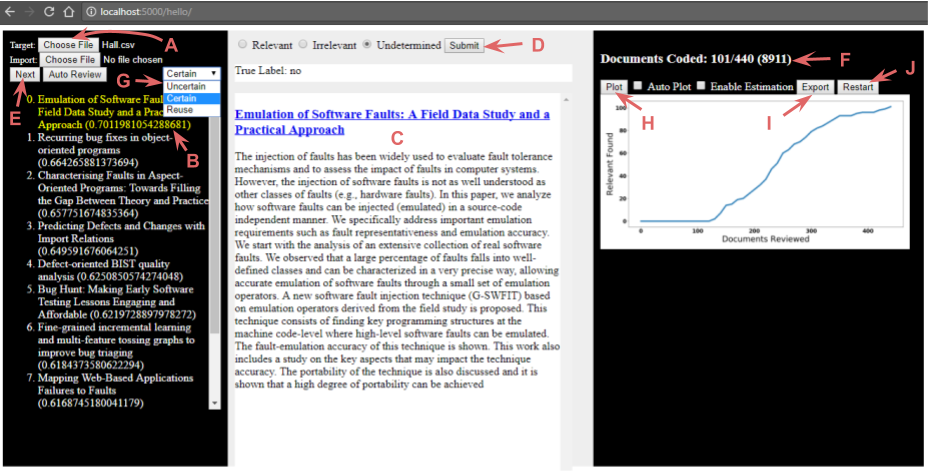
\includegraphics[width=\linewidth]{FASTREAD.png}
    \caption{Basic interface of the FASTREAD tool.}
    \label{fig:FASTREAD}
\end{figure*}


\begin{figure*}[!t]
    \centering
    \subfloat[Input format]
    {
        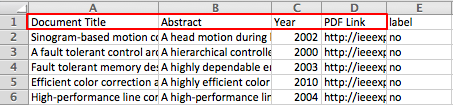
\includegraphics[width=0.48\linewidth]{Input.png}\label{fig:input}
    }
    \subfloat[Output format]
    {
        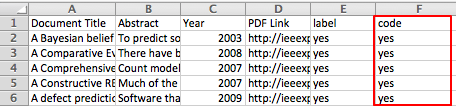
\includegraphics[width=0.48\linewidth]{Output.png}\label{fig:output}
    }    
    
    \caption{Data format for FASTREAD tool.}
    \label{fig:csv}
\end{figure*}

\section{Discussion}
\label{sect: Discussions}

\subsection{What is missed?}


Our results will show, with FASTREAD, $95\%$ of the ``relevant'' studies can be retrieved by reviewing a small portion (usually hundreds of studies) of long candidate study list. Given that, it is wise to reflect
on the 5\% of papers {\em not} found by such an analysis. To this end, we took one of our case studies and reflected on:
\begin{itemize}
\item The set of papers $R$ that a human analyst declared to be ``relevant'' (as listed in their reference list at the end of their paper);
\item The {\em tangentially relevant} subset of those  papers $R_1 \subseteq R$ that a human analyst explicitly mentions, however briefly, in the body of their paper;
\item The yet smaller subset of those papers $R_2 \subseteq R_1$  that a human analyst discusses, at length, in the body of their report (and for
our purposes ``at length'' will be ``more that two lines''). We call these {\em insightful papers}. Clearly, FASTREAD should not be recommended if our method always misses the insightful papers, 
\end{itemize}
For our case studies, on 30 repeats of our methods, we found that $R_2\setminus L_R=\emptyset$; i.e. FASTREAD never missed an insightful paper. As for the tangentially
relevant papers, FASTREAD found all of those in 95\% of the 30 repeats. 
Based on this analysis, we infer that missing  $5\%$ of the papers is not a major impediment to using FASTREAD. Similar conclusion was derived by Shemilt et al. in 2016~\cite{shemilt2016use}. \respto{1c}More interestingly, we found that more than 90\% of the missing studies come from a same set of size of $0.1|R|$. Which means some studies are more likely to be missed while most studies have never been missed in 30 repeats. This may suggest that there are outliers in relevant studies, which are not very important according to our case studies.

That said, it is still true that if the SLR conductor does not want to miss any potential relevant study, he or she need to review all the candidate studies with full cost. We are actively exploring possibilities to mitigate or compensate the missing studies issue. 
\respto{1d}For example, one technique is ``diversity sampling''; i.e. to explore unknown regions by sampling the least similar studies from what have been reviewed before. Exploration and exploitation can be balanced by selection different weight between diversity sampling and certainty/uncertainty sampling and more exploration usually means fewer missing studies but higher review cost.

% Data imbalance is explored further in Fioravanti and Nesi
% [[43]] and Zhang et al..

% Nikora and Munson [[126]] says that “without a widely agreed definition of severity
% we cannot reason about it” and Ostrand et al.
 

\subsection{What about domain knowledge?}

In our simulations, we assume that no initial seed training set is available thus a random sampling is performed to collect the minimum training set. This assumption represents the worst case while no external knowledge is available. We show in this work that the absence of that domain knowledge is not a critical failing of the approach. On the other hand, such domain knowledge usually exists in real world SLRs and will boost the performance of FASTREAD if wisely used. For example, if one relevant example and one irrelevant example are known in the very beginning, the random sampling step of FASTREAD is no longer needed and thus leads to additional cost reduction. More details about how to wisely use domain knowledge to boost FASTREAD will be explored further after this work. While we have some preliminary results in that area, we have nothing definitive to report at this time.

\subsection{What about real human reviewers?}

In our simulations, we assume that there is only one reviewer who never make mistakes. In real world SLRs, there will be multiple reviewers who make some mistakes. 

First, consider we have multiple reviewers but no mistakes. The schema of FASTREAD can be changed to one central learner with multiple review agents. Every agent reviews different studies and feedback his or her decisions to the central learner. The central learner then trains on the feedback of every agent and assigns studies to each agent for review. Such schema will keep all the property of single reviewer FASTREAD and performs similarly. In addition, there might be more intelligent way to allocate review tasks based on the different performance of review agents. Such possibility is worth exploring in future works and there already exists some studies on this topic in evidence-based medicine~\cite{wallace2011should}.

Second, consider those multiple reviewers now make mistakes. Candidate studies need to be reviewed by multiple reviewers in case any of them makes mistakes. To explore this issue, appropriate data need to be collected on how human reviewers make mistakes. Wallace et al. addressed this issue in~\cite{nguyen2015combining} by analyzing the best policy for allocating review tasks to reviewers with different experience levels as well as difference costs. We also plan to to address this issue in our future work.


\subsection{What about multiple categories of studies?}

In our simulations, we assume that the target is binary classification. However, primary study selection in real world SLRs might be a multi-label classification problem. For example, an SLR with two research questions might go through a primary study selection while each candidate is labeled as ``relevant to RQ1'', ``relevant to RQ2'', or ``irrelevant'' while the first two labels can co-exist. The simplest solution for this is to run multiple FASTREAD learners each learns on one label vs. others and each reviewer classify on one label only. In this case, the multi-label classification problem can be divided into multiple FASTREAD problems. Additional work such as ensemble learners can be explored in future works.

In summary, FASTREAD is an in-development technique that can be applied if the above trade-offs are acceptable. It can still be improved to further reduce cost of primary study selection and we will keep working on the issues until it becomes a reliable tool for different scenarios of SLRs.



\section{Threats to Validity}
\label{sect: Threats to Validity}

There are several validity threats to the design of this study~\cite{feldt2010validity}. Any conclusions made from this work must be considered with the following issues in mind:

{\em Conclusion validity} focuses on the significance of the treatment. To
enhance the conclusion validity of this work, we employed several statistical
tests (Scott-Knot) to reduce the changes of making spurious conclusions. 

{\em Internal validity} focuses on how sure we can be that the treatment
actually caused the outcome. To enhance our internal validity,
as far as possible, we heavily constrained our experiments
(see  our simulated in strictly controlled environments as discussed in Section~\ref{subsect: Controlled Variables}).

{\em Construct validity} focuses on the relation between the theory
behind the experiment and the observation. In this work, we evaluated
our results via different treatments with WSS@95 as stated in Section~\ref{subsect: Performance Metrics}-- note that those
measures took us as close as we can to computing
cost reduction without ``abstract relevant'' information. 
That is, it fits the objective of human-in-the-loop primary study selection as defined in the current literature~\cite{tredennick2015,cormack2015autonomy,cormack2014evaluation}. Increasing the number of different measures may increase construct validity
so, in future work, we will further explore more metrics.

{\em External validity }concerns how well the conclusion can be applied outside. All the conclusions in this study are drawn from the experiments running on three software engineering SLR datasets created with information from Hall, Wahono, Radjenovi{\'c} et al. studies~\cite{hall2012systematic,wahono2015systematic,radjenovic2013software} and one dataset provided by Kitchenham~\cite{kitchenham2010systematic}. Therefore, such conclusions may not be applicable to datasets of different scenarios, e.g., citation screening from evidence based medicine or TAR from e-discovery. Such bias threatens any classification experiment. The best any researcher can do is to document that bias then make available to the general research community all the materials used in a study (with the hope that other researchers will explore similar work on different datasets). Existing active learning techniques in citation screening have been criticized by Olorisade et al. for being not replicable~\cite{olorisade2016critical,olorisade2017reproducibility}. To this end, we have published all our code at \textit{https://github.com/fastread/src} and all our data at \textit{https://doi.org/10.5281/zenodo.837298}.

In the experiments, we assume that the human reviewer is always correct. In practice, this assumption cannot hold and problems such as disagreement between reviewers or concept drift (in which reviewers disagree with themselves as time passes) may occur.  As discussed
below when we discuss {\em Future Work}, we intend to explore this matter in the near future.

The comparisons in our experiment are based on the controlled variables listed in Section~\ref{sect: Controlled Variables}. The conclusion in Section~\ref{subsect: Results} may become unreliable if any of the controlled variables changes.



\section{Conclusions}\label{sect: Conclusion}

Systematic literature reviews are the primary method for aggregating evidence in evidence-based software engineering. It is suggested for every researcher in software engineering to frequently conduct SLRs in~\cite{keele2007guidelines}.
One drawback with such SLRs is the time
required to complete such a study:
  an SLR would can weeks to  months to finish and the conclusion drawn can be out of date in a few years. 
  
  To tackle this barrier to understanding the literature, this study focuses on primary study selection, one of the most difficult and time consuming steps in an SLR. Machine learning methods, especially active learning, are explored in our attempts to reduce the effort required to exclude primary studies. In this paper:
  
\begin{itemize}
\item
We explored 32 different active learners. To the best of our knowledge, this is largest
such study yet completed in the software engineering domain. 
\item
We  have collected data from four very large literature reviews. This adata is publically available at
doi.org/10.5281/zenodo.837298. Note that the creation and distribution of these data sets is a significant contribution since prior to this study, it was  very difficult to obtain even one such data set. 
\item
We have offered a baseline result that can serve
as a challenge problem for SE researchers: how to find more relevant
papers after reviewing fewer  papers. 
We  have  placed in the public domain (at github.com/fastread/src) software
tools that let others compare our approach with alternative methods.
\item
We build created a new reading-assistant tool called FASTREAD.
To the best of our knowledge, the particular combination of methods used by FASTREAD have not been previously explored.
\item
Using FASTREAD, we decreased the number of studies to be reviewed by 50\% (comparing to the prior state-of-the-art).
\end{itemize}
\newpage
\noindent
As a result  of the above we can:
\begin{itemize}
\item Offer much assistance to any future SLR;
\item Offer a cautionary tale to SE 
researchers who use data miners. Specifically: do not be content with off-the-shelf solutions developed
by other communities. SE   has nuanced differences to other domains so our methods need to be tuned to our data.
\end{itemize}


\section{Future Work}
This study has several limitations as described in Section~\ref{sect: Discussions}. ~\respto{1k}We consider the limitations as open challenges and plan to address those in future work. Specific problems and plans for the future are listed below.

\begin{itemize}

\item
{\em Conclusions are drawn from three synthetic SLR datasets and one Kitchenham dataset.} Validate the generalizability of the results on different datasets, including datasets from evidence-based medicine and e-discovery.

\item
{\em Experiment results are evaluated by WSS@95, which assumes a stop rule of reaching 95\% recall.} How to stop at 95\% recall without first knowing the number ``relevant'' studies in the pool is an interesting topic. We are exploring this topic actively.

\item
{\em The size and prevalence of data can affect performance of FASTREAD.} \respto{1b}With the capability of cost reduction from FASTREAD, it is reasonable to ask whether we need the narrow initial search. An interesting future research would be to use every paper on, say Scopus, database as candidates and allow user to just using some simple search to initiate and guide the selection. As a result, the recall is no longer restricted by the initial search string thus may yield higher recall with reasonable cost.

\item
{\em About $10\%$ to $20\%$ efforts are spent on random selection step and most of the variances are also introduced in this step.} To speed up the random selection step, external expert knowledge will be introduced while unsupervised learning methods such as \respto{1m}VTM, LDA, word2vec, or t-SNE will also be considered in future work. 

\item
{\em Some magic parameters are arbitrarily chosen, which may affect the performance.} However, parameter tuning is not a good fit for human-in-the-loop primary study selection because a) parameters should be tuned for the data working on; b) but the effect of applying different parameters can not be tested since querying extra label incurs extra cost. Therefore, novel methods should be explored for parameter selection; e.g. better criterion for when to switch from uncertainty sampling to certainty sampling (instead of the ``30'' relevant examples rule applied now).


\item
\respto{1e}{\em Current scenario is restricted to having only one reviewer, which is impractical in practice.} Problems including how to assign review tasks to multiple reviewers and how to utilize reviewers with different cost and different capability will be explored in the future.

\item
{\em Current scenario assumes that reviewers never make mistakes, which is definitely not true in practice.} How to tackle concept drift (reviewers disagree with themselves) and how to settle disagreements (reviewers disagree with each other) would be valuable contributions for future work.

\item
{\em This study focuses only on primary study selection.} Assists on other steps of SLR such as searching, data extraction, and protocol development can also help reduce total effort of SLRs. The potential of combining VTM, snowballing, and other tools with FASTREAD needs to be explored as well.


\end{itemize} We invite other researchers to join us in the exploring the above. 

% With all the work in this study, a baseline result for human-in-the-loop primary study selection has now been established. There are still many concerns and potential improvements on FASTREAD, as discussed in Section~\ref{sect: Frequently Asked Questions}. We will keep working on the future work items and we believe that with all the materials in this work published, SE researchers can also explore further in SLR cost reduction. With our best hope, the effort required for conducting SLRs will eventually be reduced to days of work in the future and thus enable researchers to conduct SLRs much more frequently.

\section*{Acknowledgement}
The authors thank Barbara Kitchenham for
her attention to this work and for
sharing with us the ``Kitchenham'' dataset used in our experiments.
 
% \bibliographystyle{plain}
\bibliographystyle{spmpsci}
\bibliography{sigproc} 






\appendix 


\newpage
\normalsize
\section*{Response to Reviewers}

Reviewer comments are shown {\em in italics} and our replies
are offered in plain text.

\subsection*{Comments from the coordinating editor}

\review{The revised manuscript is reviewed by the same three reviewers as before. The detailed questions are judged being properly handled, although there are still concerns with the contribution and presentation. }


Please thank all the reviewers for their careful comments. 

Based on your comments, we have significantly reorganized, clarified and shortened this draft.

Please note that there is no new semantic content in this new draft. With one exception, the order of the content is same  (and that content is now expressed much more clearly and succinctly). That exception is that the new Section 7 contains material that, previously, was earlier in the paper.

We hope this can be processed  as a “minor review” (i.e. reviewed by A/Editor).

Replies to your specific comments are offered below.
Before that, we note that Reviewer \#3 remains critical saying ``In fact, it is just a comparison of performance of several algorithms'' That is a valid comment to be sure  but , with respect, it does not do justice to the effort
associated with this paper, nor the insights achieved with
this work, by ``just'' achieving this result. Please consider what  we ``just'' achieved in this paper:
\begin{itemize}
\item
We explored 32 different active learners. To the best of our knowledge, this is largest
such study yet completed in the software engineering domain. 
\item
We  have collected data from four very large literature reviews. This adata is publically available at
doi.org/10.5281/zenodo.837298. Note that the creation and distribution of these data sets is a significant contribution since prior to this study, it was  very difficult to obtain even one such data set. 
\item
We have offered a baseline result that can serve
as a challenge problem for SE researchers: how to find more relevant
papers after reviewing fewer  papers. 
We  have  placed in the public domain (at github.com/fastread/src) software
tools that let others compare our approach with alternative methods.
\item
We build created a new reading-assistant tool called FASTREAD.
To the best of our knowledge, the particular combination of methods used by FASTREAD have not been previously explored.
\item
Using FASTREAD, we decreased the number of studies to be reviewed by 50\% (comparing to the prior state-of-the-art).
\end{itemize}
As a result  of the above we can:
\begin{itemize}
\item Offer much assistance to any future SLR;
\item Offer a cautionary tale to SE 
researchers who use data miners. Specifically: do not be content with off-the-shelf solutions developed
by other communities. SE   has nuanced differences to other domains so our methods need to be tuned to our data.
\end{itemize}
In our opinion, this is more than just enough to merit publication. But what is your view?

\par~

\noindent
\newpage
As to your specific comments:
\begin{itemize}
\item
\review{\textbf{R0-a:} The authors are advised to take a step back and rethink the manuscript and clarify what is the core contribution to the SE community.}

Please check our new introduction-- we think it makes "the point" much more clearly.
\par~

\item
\review{\textbf{R0-b:} The advertising style of the paper makes it hard to assess what is new, as it is overselling the contributions.}

This is a good point-- we hope our new title and  the new (much condensed)   introduction addresses your point.
\par~

\item
\review{\textbf{R0-c:} Already the title uses value words “On the benefits…” The abstract tells that FASTREAD “outperformed current methods” and saves “much time”. Academic papers should be more precise and value neutral.}

We have rewritten the  abstract introduction, as per your direction. The new abstract of the new draft is much more precise, we think.

\par~

\item
\review{\textbf{R0-d:} We foresee a significantly revised manuscript, which clearly and openly presents the contribution and the outcomes.}

The new version is significantly re-organized.  E.g. this new draft is fully six pages shorter; large sections have moved to the back; one confusing set of results (relating to “domination”) have been discarded; the abstract and introduction have been completely rewritten. 

Also, at your direction, the contributions and outcomes are now presented very clearly and succinctly in the introduction. The precise numerical results are now presented, in the abstract and  before the end of our introduction (\citeresp{0d}):
\par~

\item
\review{\textbf{R0-e:} The authors should clarify this paper’s key contribution.}

Thanks for this comment, we have clarified our contribution in the introduction and included the literature~\cite{ros2017machine} in related works~\citeresp{0e}.
\par~
\item
\review{\textbf{R0-f:} Try to find a way to let the results speak for themselves, rather than arguing for their uniqueness and novelty. Perhaps design science research may be a framework to present the work in, that elaborates on the problem identification (SLRs are time consuming), the design of the solution (FASTREAD), and the evaluation of the solution (replication of SLRs) are three parts that together make up the contribution of the manuscript. Hevner’s design, relevance and rigor cycles match the three items above well (A. R. Hevner, S. T. March, J. Park, and S. Ram. Design science in information systems research. MIS Q., 28(1):75–105, Mar. 2004.)}

Thanks for this comment, we have re-organized this paper to better match this pattern. We think the new title serves that purpose (what do you think?).
\par~
\item
\review{\textbf{R0-g:}  The unconventional writing of the paper contributes to the mixed responses. Section titles like "Frequently asked questions" and "Technical notes" indicate rather material that should belong to an appendix than being part of the main flow of the paper.}

Good point. We have removed those unnecessary conflations.
\par~

\end{itemize}








 



\subsection*{Response to Reviewer \#1}

\review{ I believe all my previous comments were sufficiently addressed. I do not agree with everything, but that is not a necessity. First of I should say that I would use this tool if I would do an SLR, if it is possible to tweak it according to my preferences in starting set. It must be possible to change previous classifications, due to concept drift or miss-classifications.}

Thank you for those comments. We revised this paper based on all the comments and believe that it is much improved. FYI, the FASTREAD tool has been updated a lot since the submission of this paper, the latest version\footnote{https://github.com/fastread/src} does include features allowing user to tweak starting set, hint of remaining relevant studies and change previous classifications.
\par ~

%%%%%%%%%%%%%%%%%%%%
% Review 1a
%%%%%%%%%%%%%%%%%%%%
\review{\textbf{R1-a:} Your statistical analysis with medians and dominance is unconvential and produces very awkward tables, I am not sure that it is valid. It is problematic when one factor is not strictly dominated by another, should you then select by highest number of domination? Do you have any theoretical justification for that? When using ANOVA you have a much easier time when asking questions about specific factors in the treatment. You are right to question the assumptions of ANOVA, which is that the residuals are normally distributed, which can occur when the response variable is not normally distributed. ANOVA is also quite robust against the normality assumptions, instead equal variance in all populations is the tricky assumption in ANOVA. There are other alternatives to factorial ANOVA that might not be non-parametric, but at least robust, which is what you are really looking for, e.g. Van der Waerden test/Normal Scores test. Another alternative is to only consider what the best
result is, i.e. only Scott-Knott analysis. Though that necessitate removing the research questions on factors RQ2.1-RQ2.4.
}

This is a very good point. Based on your comment, we performed a ``what-if'' study. Specifically, we looked to see what would happen if we just deleted all the domination results you discussed above. We found that the added complexity of that analysis was just not worth the trouble required to explain it. Hence, we just dropped it. 

Thank you for prompting that simplification.

\par ~

%%%%%%%%%%%%%%%%%%%%
% Review 1b
%%%%%%%%%%%%%%%%%%%%
\review{\textbf{R1-b:} Since my previous review I have thought of an issue that effects this work. A philosophical problem is the premise that tool assisted reviews need to be less than or equal to manual reviews, in terms of studies found. Whenever tool assistance is successful it is because they enable a different workflow. For your tool, the only selling point is saved time. You should have a discussion on whether you could instead have a wider search string than what you would have for a manual review. Of course it is the case that search strings usually do not have 100\% recall, with no way of really knowing this.
}

That is a very interesting idea. And one that touches on issues that requires a new paper. With your permission, we would prefer to focus on that matter in subsequent work~\citeresp{1b}.

For now, we’d just like to say that “only” saving time is a big selling point. We work with commercial text mining companies who sell this kind of technology via the business case that saving time is a very big  saving, indeed. FYI: Over two-thirds of the costs of large legal cases is the cost of running  a basement of paralegals reading 1000s to 10,000s of documents. 

%%%%%%%%%%%%%%%%%%%%
% Review 1c
%%%%%%%%%%%%%%%%%%%%

\review{\textbf{R1-c:} Section 2.2 has a discussion on relevant/influential papers. As far as I understand, your techniques do not have any way to actually detect this. The only feasible way to detect influential studies is through citation analysis. So whether the relevant studies are included in the 95\% or not is just luck. What am I missing here?
}

We agree with you that there is no guarantee of not missing an important study. However, there are evidences that some studies are more likely to be missed while most studies have never been missed in 30 repeats~\citeresp{1c}. This may suggest that there are outliers in relevant studies, which are not very important according to our case studies. Also, Shemilt et al. found the similar results in 2016~\cite{shemilt2016use}.
 \par ~
 

%%%%%%%%%%%%%%%%%%%%
% Review 1d
%%%%%%%%%%%%%%%%%%%%
\review{\textbf{R1-d:} In section 2.2 you mention that you are actively exploring possibilities to mitigate or compensate the missing studies issue. Is this even possible? I think you should include some hints on this, or you leave the reader wondering.
}

We think what you have suggested in \textbf{R1-b} is one possible way to compensate the missing studies-- by including more candidates in the beginning and hopefully find more relevant. Other possible ways might be putting more effort on exploration instead of exploitation~\citeresp{1d}.

\par ~

%%%%%%%%%%%%%%%%%%%%
% Review 1e
%%%%%%%%%%%%%%%%%%%%
\review{\textbf{R1-e:} It would be interesting to use your tool in parallel by two reviewers and see what differences there are in the learned models that the two reviewers construct. This could be a potential use for this technology, since this comparison could be done in "large scale", where a typical manual comparison is just a few papers because of the cost associated with double reviewing.}

We completely agree~\citeresp{1e}. We are currently exploring options for using FASTREAD with multiple reviewers who might disagree with each other. What we found (from our preliminary results) is that model learned from FASTREAD can in return help resolving disagreements of reviewers. But that is work under-development and we have nothing definitive to offer on that point at this time.
\par ~

%%%%%%%%%%%%%%%%%%%%
% Review 1f
%%%%%%%%%%%%%%%%%%%%

\review{\textbf{R1-f:} Section 3, page 6. To be fair, research is never impossible, but publishing said research is impossible without background knowledge.}

Text removed.


\par ~

%%%%%%%%%%%%%%%%%%%%
% Review 1g
%%%%%%%%%%%%%%%%%%%%

\review{\textbf{R1-g:} Fig. 4, page 10. These illustrations are illuminating. You do not explain that the axis represent a simplified problem with just two features. You should visually distinguish between excluded papers and yet unlabeled examples, especially in (b).}

Illustration improved on that figure~\citeresp{1g}.
\par~

%%%%%%%%%%%%%%%%%%%%
% Review 1h
%%%%%%%%%%%%%%%%%%%%

\review{\textbf{R1-h:} Section 4.2, page 10. You should mention the main drawback to SVM in this context, it is hard to inspect what the model has learned.}

Drawback of SVM added~\citeresp{1h}.
\par~

%%%%%%%%%%%%%%%%%%%%
% Review 1i
%%%%%%%%%%%%%%%%%%%%

\review{\textbf{R1-i:} Section 4.3. It is commonly believed by who? Could you mention a citation? Besides, I thought the goal of this work was to find papers as fast as possible, not gaining information. I don't think it is as obvious as you think that uncertainty sampling is better than certainty sampling.}

Text removed, no longer applicable.
\par~

%%%%%%%%%%%%%%%%%%%%
% Review 1j
%%%%%%%%%%%%%%%%%%%%

\review{\textbf{R1-j:} Page 18. Now you are over hedging your claim, based on the most realistic data set in your evaluation (Kitchenham) you can at least say 50\% reduction. I think this figure is more realistic, given that a normal reviewer attempts to reduce the scope as much as possible, by tuning the search string or adding filters, to reduce manual work.}

RQ3 now provides more details on how much effort can be saved by FASTREAD~\citeresp{1j}.
\par~

%%%%%%%%%%%%%%%%%%%%
% Review 1k
%%%%%%%%%%%%%%%%%%%%

\review{\textbf{R1-k:} Page 25. You mention in your comments that you consider the future work as open challenges in this field, you should make that clear in section 10 as well (in the opening paragraph).}

Added into Section 10, opening paragraph~\citeresp{1k}.
\par~

%%%%%%%%%%%%%%%%%%%%
% Review 1l
%%%%%%%%%%%%%%%%%%%%

\review{\textbf{R1-l:} On future work, I would discourage you from pursuing the stopping criterion direction. Visual indications is good enough in my opinion, are you doing this just for the sake of being systematic? Or is there an actual need of an objective stopping criterion?}

Totally agree with you. We are exploring this issue by building an estimator of how many relevant studies remains in the unlabeled set. Results are promising and as you suggested, it is not a hard stopping criterion, but an indicator that helps user to decide whether to stop or not. If you are interested, please follow us on our future publications or try the latest version of FASTREAD tool.
\par~

%%%%%%%%%%%%%%%%%%%%
% Review 1m
%%%%%%%%%%%%%%%%%%%%

\review{\textbf{R1-m:} Also, LDA for text classification is outdated, go with word2vec, which is available in scikit-learn. It is also commonly used with t-SNE for visualisations, which could be an interesting visualization for reviewers.}

We will not say LDA is outdated but thanks for your suggestions and we will definitely explore the mentioned latest techniques~\citeresp{1m}.
\par~

%%%%%%%%%%%%%%%%%%%%
% Review 1n
%%%%%%%%%%%%%%%%%%%%

\review{\textbf{R1-n:} Minor comments and grammatical errors.}

Thanks for your careful read. All minor points and grammatical errors fixed.
\par~


\subsection*{Response to Reviewer \#3}

\review{Thank you for your revised version. It is clear that you put a lot of effort in this revision and several issues have been properly addressed. However, my main criticisms against the work were not addressed satisfactorily.}

Thanks for your review. Please find the responses to the detailed comments below.
\par ~

%%%%%%%%%%%%%%%%%%%%
% Review 3a
%%%%%%%%%%%%%%%%%%%%
\review{\textbf{R3-a:} Small sample size X generalization: adding 2 more data points is not enough to improve external validity. Further, it is not a case of simply dropping the claim of 90\% reduction. The problem here is related to whatever generalization claim you make with this tiny number of data points. Further yet, the reasons for choosing these SLRs was not explained, that is, the sampling method was not clearly defined and sampling can bias the results. This was not properly discussed in your revision.}

Thank you for your comment. We have been researching this area for three years now and can assert that most of these tools are tested using very little public domain data, indeed.  Hence we say that~\citeresp{3a}:
\begin{itemize}
\item
The creation and distribution of these data sets (by this paper) is a significant contribution since prior to this study, it was very difficult to obtain even one such data set.
\end{itemize}
Now we agree with you that, ideally,  this kind of work should be assessed using more data. But how to acquire that data? As we say here, it is very hard to collect. One strategy is to publish one paper using whatever data is available (and with that paper, publish all the tools needed to comparatively assess new active learning methods). That is, by publishing this paper, we can move this research sub-field towards the goal you desire.

\par ~

%%%%%%%%%%%%%%%%%%%%
% Review 3b
%%%%%%%%%%%%%%%%%%%%
\review{\textbf{R3-b:} Relevance: as I mentioned in my first review, this study only shows that a certain algorithm outperform others in on of the many steps in study selection in SLR. The solution was not tested against other types of search/selection processes/tools. Therefore, I am still concerned about the overall relevance of this study to improve SLR in SE.}

With respect, we must disagree on this point. We would assert that FASTREAD has been  extensively ``tested against other types of search/selection processes/tools''. To build FASTREAD,  we read \textit{everything} we could find on automated assisted reviewing. We pulled those other methods apart and implemented their 32 subroutines. We tried them all to achieve the results in this paper. 

Perhaps what you meant to say was that   Figure~\ref{fig:barrier} of this paper describes eight  parts of systematic reviews and this paper only explores one part (primary selection study). If so, we would direct you to the first parts of section~\ref{sect: sect2} where we note that some of these eight  parts already have tool support. Also, regarding primary selection study, we note that the survey reported in Fig1 shows that primary selection study is widely agreed to be one of the most difficult and most time consuming parts of SLRs.  That is why we study this one part of SLRs.

\par ~

%%%%%%%%%%%%%%%%%%%%
% Review 3c
%%%%%%%%%%%%%%%%%%%%
\review{\textbf{R3-c:} List of future work versus study limitations: I was not clear when I pointed out in my first review that the study is still immature as many important issues were listed as future work. I do agree with the authors that pointing out directions for future research is very important par of any relevant academic publication. I was not talking about future work, but as limitation of this study that were listed as things to be dealt with in the future. Some limitations can indeed be addressed as part of future research, but some are just limitations that make the work immature and not fit for publication as is. For instance, small number of data points impacting generalizability of the study cannot simply be pushed forward for future studies as it is a major threat to validity and relevance of your study. Further, "The size and prevalence of data can affect performance of FASTREAD" and so this can invalidate the results in other data sets in SE; thus, how can I trust that using FASTREAD next time will actually be any good?}

That’s a valid perspective but respectfully, we do not think it precludes publication. 

We do not think it is bad practice to clearly state the limits of a study.  

What we do think is good practice is to put out all tools and data sets and publish some baselines such that the research community in general can work to improve our results. Hence, this paper.

We also think that what was achieved with FASTREAD is head and shoulders above anything done before (in SE, and other fields). Please look at our results--- much better than the prior state of the art seen in PCTW, PUSA, HCTN.



\par ~

%%%%%%%%%%%%%%%%%%%%
% Review 3*
%%%%%%%%%%%%%%%%%%%%
\review{Three of my major concerns regarding this study were not addressed properly. Therefore, I am keeping the general conclusion of my first review: In summary, there is nothing particularly new about the study design to make this study compelling for publication for its methodological aspects. In fact, it is just a comparison of performance of several algorithms and the experimental design has several problems as commented above. Further, it is not clear how relevant the studies are in supporting the SLR development. The proposed tool was not tested against alternative selection techniques or even against humans. So, the contribution is very small for publication in EMS.}


This is a valid comment to be sure  but , with respect, it does not do justice to the effort
associated with this paper, nor the insights achieved with
this work, by ``just'' achieving this result. Please consider what  we ``just'' achieved in this paper:
\begin{itemize}
\item
We explored 32 different active learners. To the best of our knowledge, this is largest
such study yet completed in the software engineering domain. 
\item
We  have collected data from four very large literature reviews. This adata is publically available at
doi.org/10.5281/zenodo.837298. Note that the creation and distribution of these data sets is a significant contribution since prior to this study, it was  very difficult to obtain even one such data set. 
\item
We have offered a baseline result that can serve
as a challenge problem for SE researchers: how to find more relevant
papers after reviewing fewer  papers. 
We  have  placed in the public domain (at github.com/fastread/src) software
tools that let others compare our approach with alternative methods.
\item
We build created a new reading-assistant tool called FASTREAD.
To the best of our knowledge, the particular combination of methods used by FASTREAD have not been previously explored.
\item
Using FASTREAD, we decreased the number of studies to be reviewed by 50\% (comparing to the prior state-of-the-art).
\end{itemize} As a result  of the above we can:
\begin{itemize}
\item Offer much assistance to any future SLR;
\item Offer a cautionary tale to SE 
researchers who use data miners. Specifically: do not be content with off-the-shelf solutions developed
by other communities. SE   has nuanced differences to other domains so our methods need to be tuned to our data.
\end{itemize}

\end{document}


